\documentclass[twocolumn]{article}

% Import required packages
\usepackage{preprint}
\usepackage[utf8]{inputenc}
\usepackage[T1]{fontenc}
\usepackage{amsmath, amsthm, amssymb, amsfonts}
\usepackage{graphicx}
\usepackage[numbers,square]{natbib}
\usepackage{subcaption}
\usepackage{booktabs}
\usepackage{float}
\usepackage{geometry}
\usepackage{xcolor}
\usepackage[colorlinks = true,
            linkcolor = purple,
            urlcolor  = blue,
            citecolor = cyan,
            anchorcolor = black]{hyperref}
\usepackage{microtype}
\usepackage{lineno}
\usepackage{titlesec}

% Adjust page geometry and spacing
\geometry{margin=2.5cm}
\setlength{\columnsep}{20pt}
\setlength{\parskip}{6pt}
\setlength{\parindent}{15pt}
\setlength{\headheight}{16.0pt}
\setlength{\footskip}{3.6pt}
\addtolength{\topmargin}{-5.15994pt}

% Section title spacing
\titlespacing\section{0pt}{12pt plus 3pt minus 3pt}{1pt plus 1pt minus 1pt}
\titlespacing\subsection{0pt}{10pt plus 3pt minus 3pt}{1pt plus 1pt minus 1pt}
\titlespacing\subsubsection{0pt}{8pt plus 3pt minus 3pt}{1pt plus 1pt minus 1pt}

% Configure graphics path
\graphicspath{
    {img/tulsi/}
    {img/lemone/}
    {img/mango/}
    {img/money/}
    {img/rosa/}
    {pics/}
}

% Add watermark with submission status
\usepackage{xwatermark}
% Bottom watermark
\newwatermark[firstpage,color=gray!90,angle=0,scale=0.28, xpos=0in,ypos=-5in]{*correspondence: \texttt{kishan.patel@amcst.edu.in}}

% Document information
\title{\Large Leaf Classification Using A Custom CNN}

\usepackage{authblk}
\renewcommand*{\Authfont}{\bfseries}
\author[1\thanks{\tt{kishan.patel@amcst.edu.in}}]{Kishan Patel}
\author[1]{Jayesh Shinde}
\author[1]{Meghraj Patel}
\author[1]{Jash Dhimmar}
\affil[1]{Asha M Tarsadia Institute of Computer Science and Technology}

\date{\today}

\begin{document}

\twocolumn[
  \begin{@twocolumnfalse}
    \maketitle

    \begin{abstract}
    \noindent
    This research focuses on developing a deep learning model for classifying five species of Indian herbal plant leaves: Lemon, Tulsi, Mango, Money Plant, and Rosa-senensis using a custom Convolutional Neural Network (CNN). The study utilizes a dataset of 5000 images (1000 per class) with 128x128 pixel resolution. The model architecture consists of multiple convolutional layers with ReLU activation and pooling layers, achieving a test accuracy of 91.1\%. The results demonstrate the effectiveness of the custom CNN in leaf classification, with potential applications in botanical research and agriculture.
    \end{abstract}
    \vspace{0.35cm}
  \end{@twocolumnfalse}
]

% Enable line numbers for the main text
\linenumbers

\section{Introduction}
The classification of plant leaves is crucial for various applications in botany, agriculture, and environmental studies. Traditional methods of leaf classification rely heavily on manual expertise and are time-consuming. Deep learning approaches \cite{lecun2015deep} have revolutionized computer vision tasks, particularly through Convolutional Neural Networks (CNNs) \cite{krizhevsky2012imagenet}. Recent studies have demonstrated the effectiveness of CNNs in plant species classification \cite{wu2019plant, pawara2017comparing}. This research presents an automated approach using deep learning techniques to classify five species of Indian herbal plant leaves, building upon the architectural principles established by pioneering works in the field \cite{simonyan2014very}.

\section{Methods}
\subsection{Dataset}
The dataset comprises:
\begin{itemize}\itemsep4pt
    \item Total Images: 5000 (1000 per class)
    \item Image Size: 128x128 pixels
    \item Classes: Lemon, Tulsi, Mango, Money Plant, Rosa-senensis
    \item Train-Test Split: 70-30\%
\end{itemize}

\subsection{Sample Images}
\begin{figure}[H]
    \centering
    \begin{subfigure}[b]{0.30\columnwidth}
        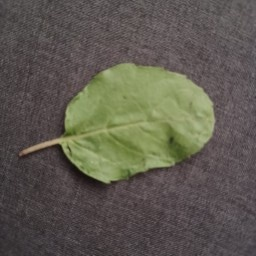
\includegraphics[width=\textwidth]{tulsi1}
    \end{subfigure}
    \hfill
    \begin{subfigure}[b]{0.30\columnwidth}
        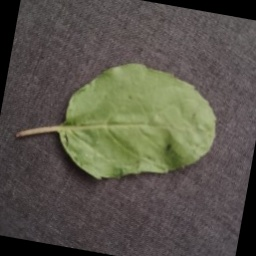
\includegraphics[width=\textwidth]{tulsi2}
    \end{subfigure}
    \hfill
    \begin{subfigure}[b]{0.30\columnwidth}
        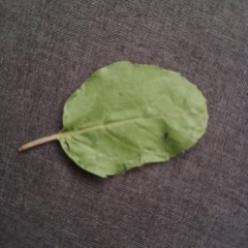
\includegraphics[width=\textwidth]{tulsi3}
    \end{subfigure}
    \vspace{0.5em}
    
    \begin{subfigure}[b]{0.30\columnwidth}
        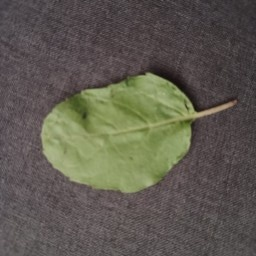
\includegraphics[width=\textwidth]{tulsi4}
    \end{subfigure}
    \hfill
    \begin{subfigure}[b]{0.30\columnwidth}
        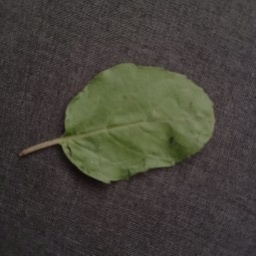
\includegraphics[width=\textwidth]{tulsi5}
    \end{subfigure}
    \hfill
    \begin{subfigure}[b]{0.30\columnwidth}
        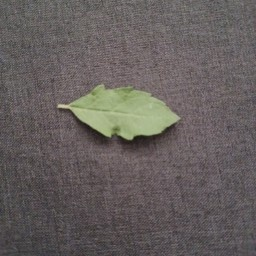
\includegraphics[width=\textwidth]{tulsi6}
    \end{subfigure}
    \vspace{0.5em}
    
    \begin{subfigure}[b]{0.30\columnwidth}
        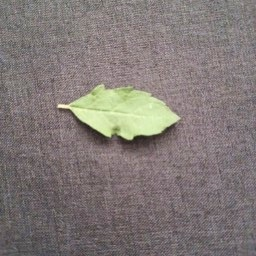
\includegraphics[width=\textwidth]{tulsi7}
    \end{subfigure}
    \hfill
    \begin{subfigure}[b]{0.30\columnwidth}
        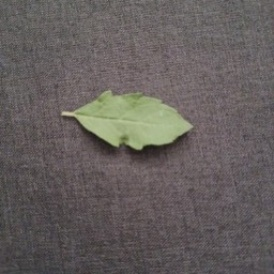
\includegraphics[width=\textwidth]{tulsi8}
    \end{subfigure}
    \hfill
    \begin{subfigure}[b]{0.30\columnwidth}
        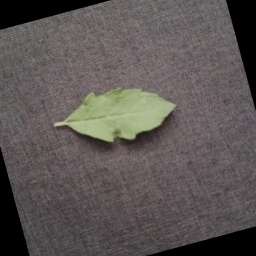
\includegraphics[width=\textwidth]{tulsi9}
    \end{subfigure}
    \caption{Sample Tulsi leaves from the dataset}
    \label{fig:tulsi-samples}
\end{figure}

\begin{figure}[H]
    \centering
    \begin{subfigure}[b]{0.30\columnwidth}
        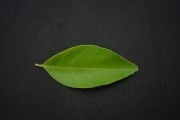
\includegraphics[width=\textwidth]{lemon1}
    \end{subfigure}
    \hfill
    \begin{subfigure}[b]{0.30\columnwidth}
        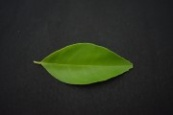
\includegraphics[width=\textwidth]{lemon2}
    \end{subfigure}
    \hfill
    \begin{subfigure}[b]{0.30\columnwidth}
        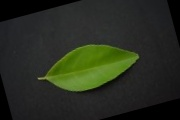
\includegraphics[width=\textwidth]{lemon3}
    \end{subfigure}
    \vspace{0.5em}
    
    \begin{subfigure}[b]{0.30\columnwidth}
        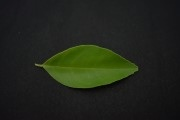
\includegraphics[width=\textwidth]{lemon4}
    \end{subfigure}
    \hfill
    \begin{subfigure}[b]{0.30\columnwidth}
        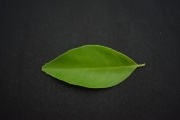
\includegraphics[width=\textwidth]{lemon5}
    \end{subfigure}
    \hfill
    \begin{subfigure}[b]{0.30\columnwidth}
        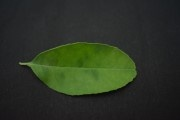
\includegraphics[width=\textwidth]{lemon6}
    \end{subfigure}
    \vspace{0.5em}
    
    \begin{subfigure}[b]{0.30\columnwidth}
        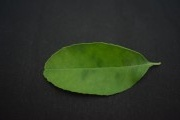
\includegraphics[width=\textwidth]{lemon7}
    \end{subfigure}
    \hfill
    \begin{subfigure}[b]{0.30\columnwidth}
        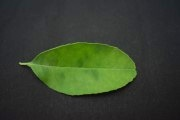
\includegraphics[width=\textwidth]{lemon8}
    \end{subfigure}
    \hfill
    \begin{subfigure}[b]{0.30\columnwidth}
        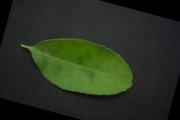
\includegraphics[width=\textwidth]{lemon9}
    \end{subfigure}
    \caption{Sample Lemon leaves from the dataset}
    \label{fig:lemon-samples}
\end{figure}

\begin{figure}[H]
    \centering
    \begin{subfigure}[b]{0.30\columnwidth}
        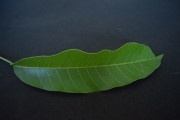
\includegraphics[width=\textwidth]{mango1}
    \end{subfigure}
    \hfill
    \begin{subfigure}[b]{0.30\columnwidth}
        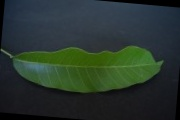
\includegraphics[width=\textwidth]{mango2}
    \end{subfigure}
    \hfill
    \begin{subfigure}[b]{0.30\columnwidth}
        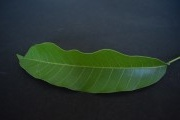
\includegraphics[width=\textwidth]{mango3}
    \end{subfigure}
    \vspace{0.5em}
    
    \begin{subfigure}[b]{0.30\columnwidth}
        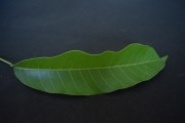
\includegraphics[width=\textwidth]{mango4}
    \end{subfigure}
    \hfill
    \begin{subfigure}[b]{0.30\columnwidth}
        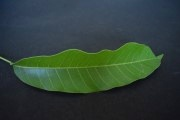
\includegraphics[width=\textwidth]{mango5}
    \end{subfigure}
    \hfill
    \begin{subfigure}[b]{0.30\columnwidth}
        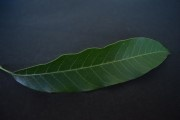
\includegraphics[width=\textwidth]{mango6}
    \end{subfigure}
    \vspace{0.5em}
    
    \begin{subfigure}[b]{0.30\columnwidth}
        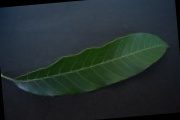
\includegraphics[width=\textwidth]{mango7}
    \end{subfigure}
    \hfill
    \begin{subfigure}[b]{0.30\columnwidth}
        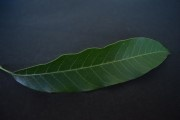
\includegraphics[width=\textwidth]{mango8}
    \end{subfigure}
    \hfill
    \begin{subfigure}[b]{0.30\columnwidth}
        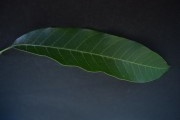
\includegraphics[width=\textwidth]{mango9}
    \end{subfigure}
    \caption{Sample Mango leaves from the dataset}
    \label{fig:mango-samples}
\end{figure}

\begin{figure}[H]
    \centering
    \begin{subfigure}[b]{0.30\columnwidth}
        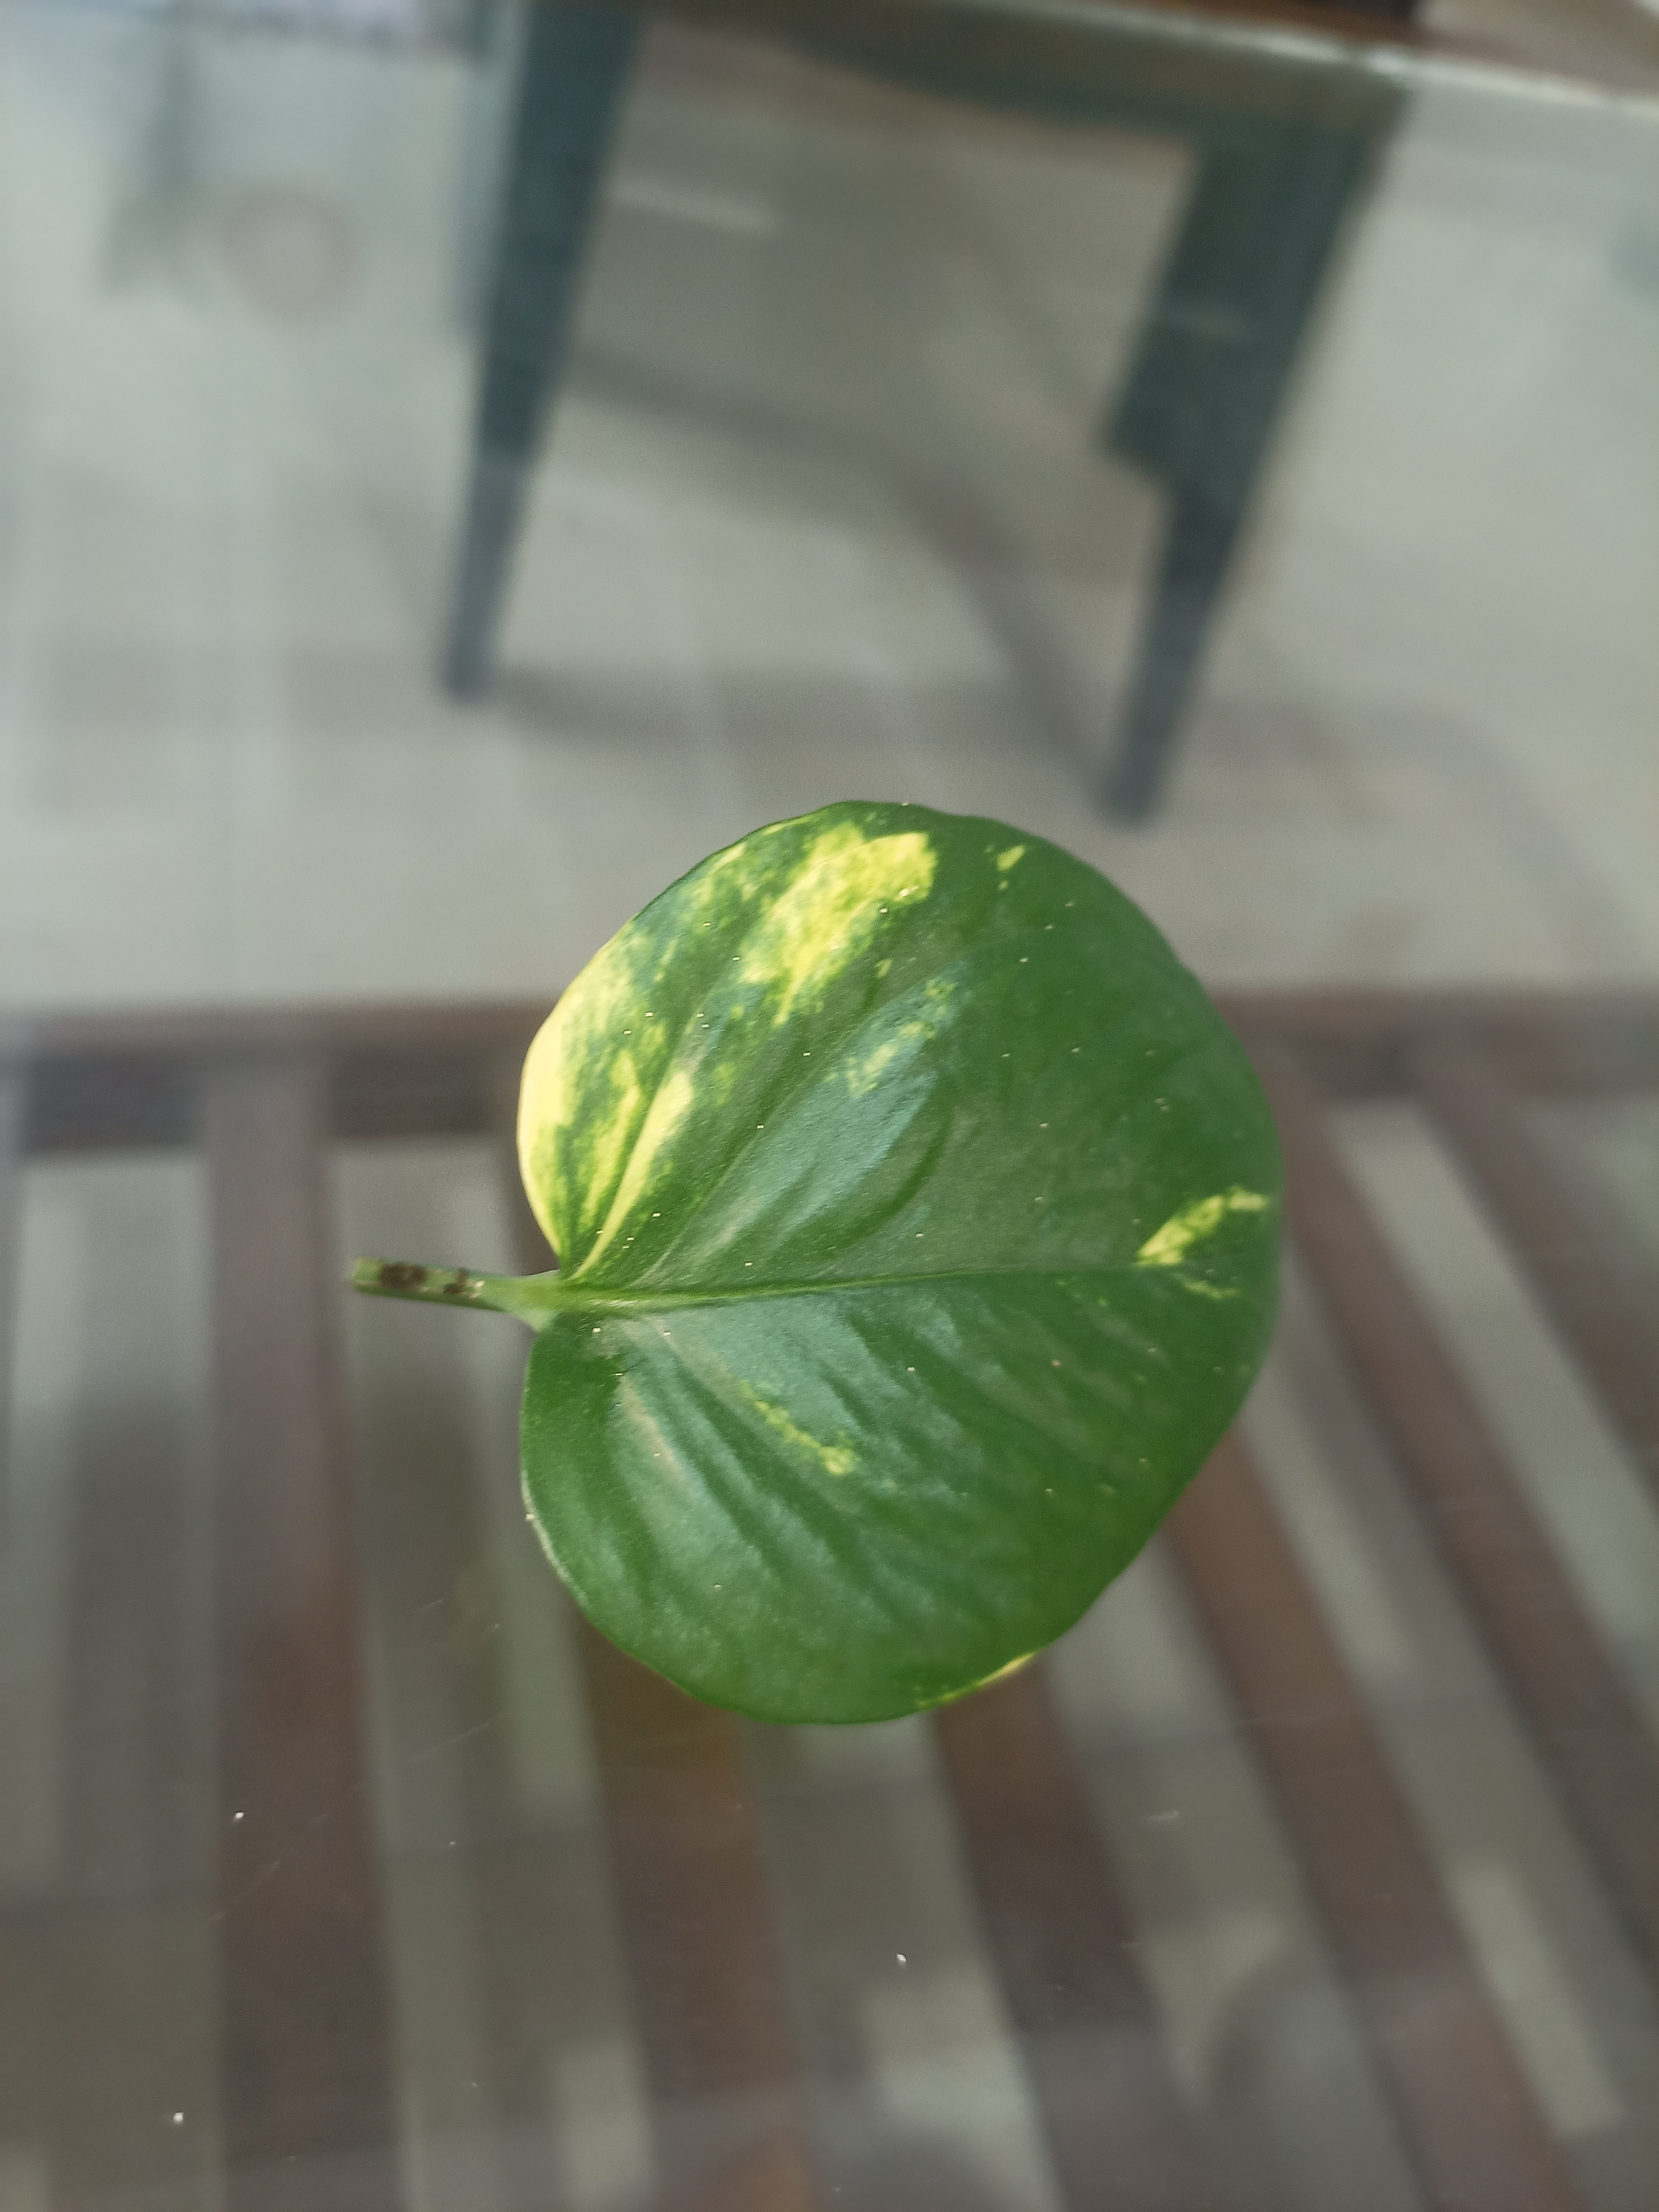
\includegraphics[width=\textwidth]{money1}
    \end{subfigure}
    \hfill
    \begin{subfigure}[b]{0.30\columnwidth}
        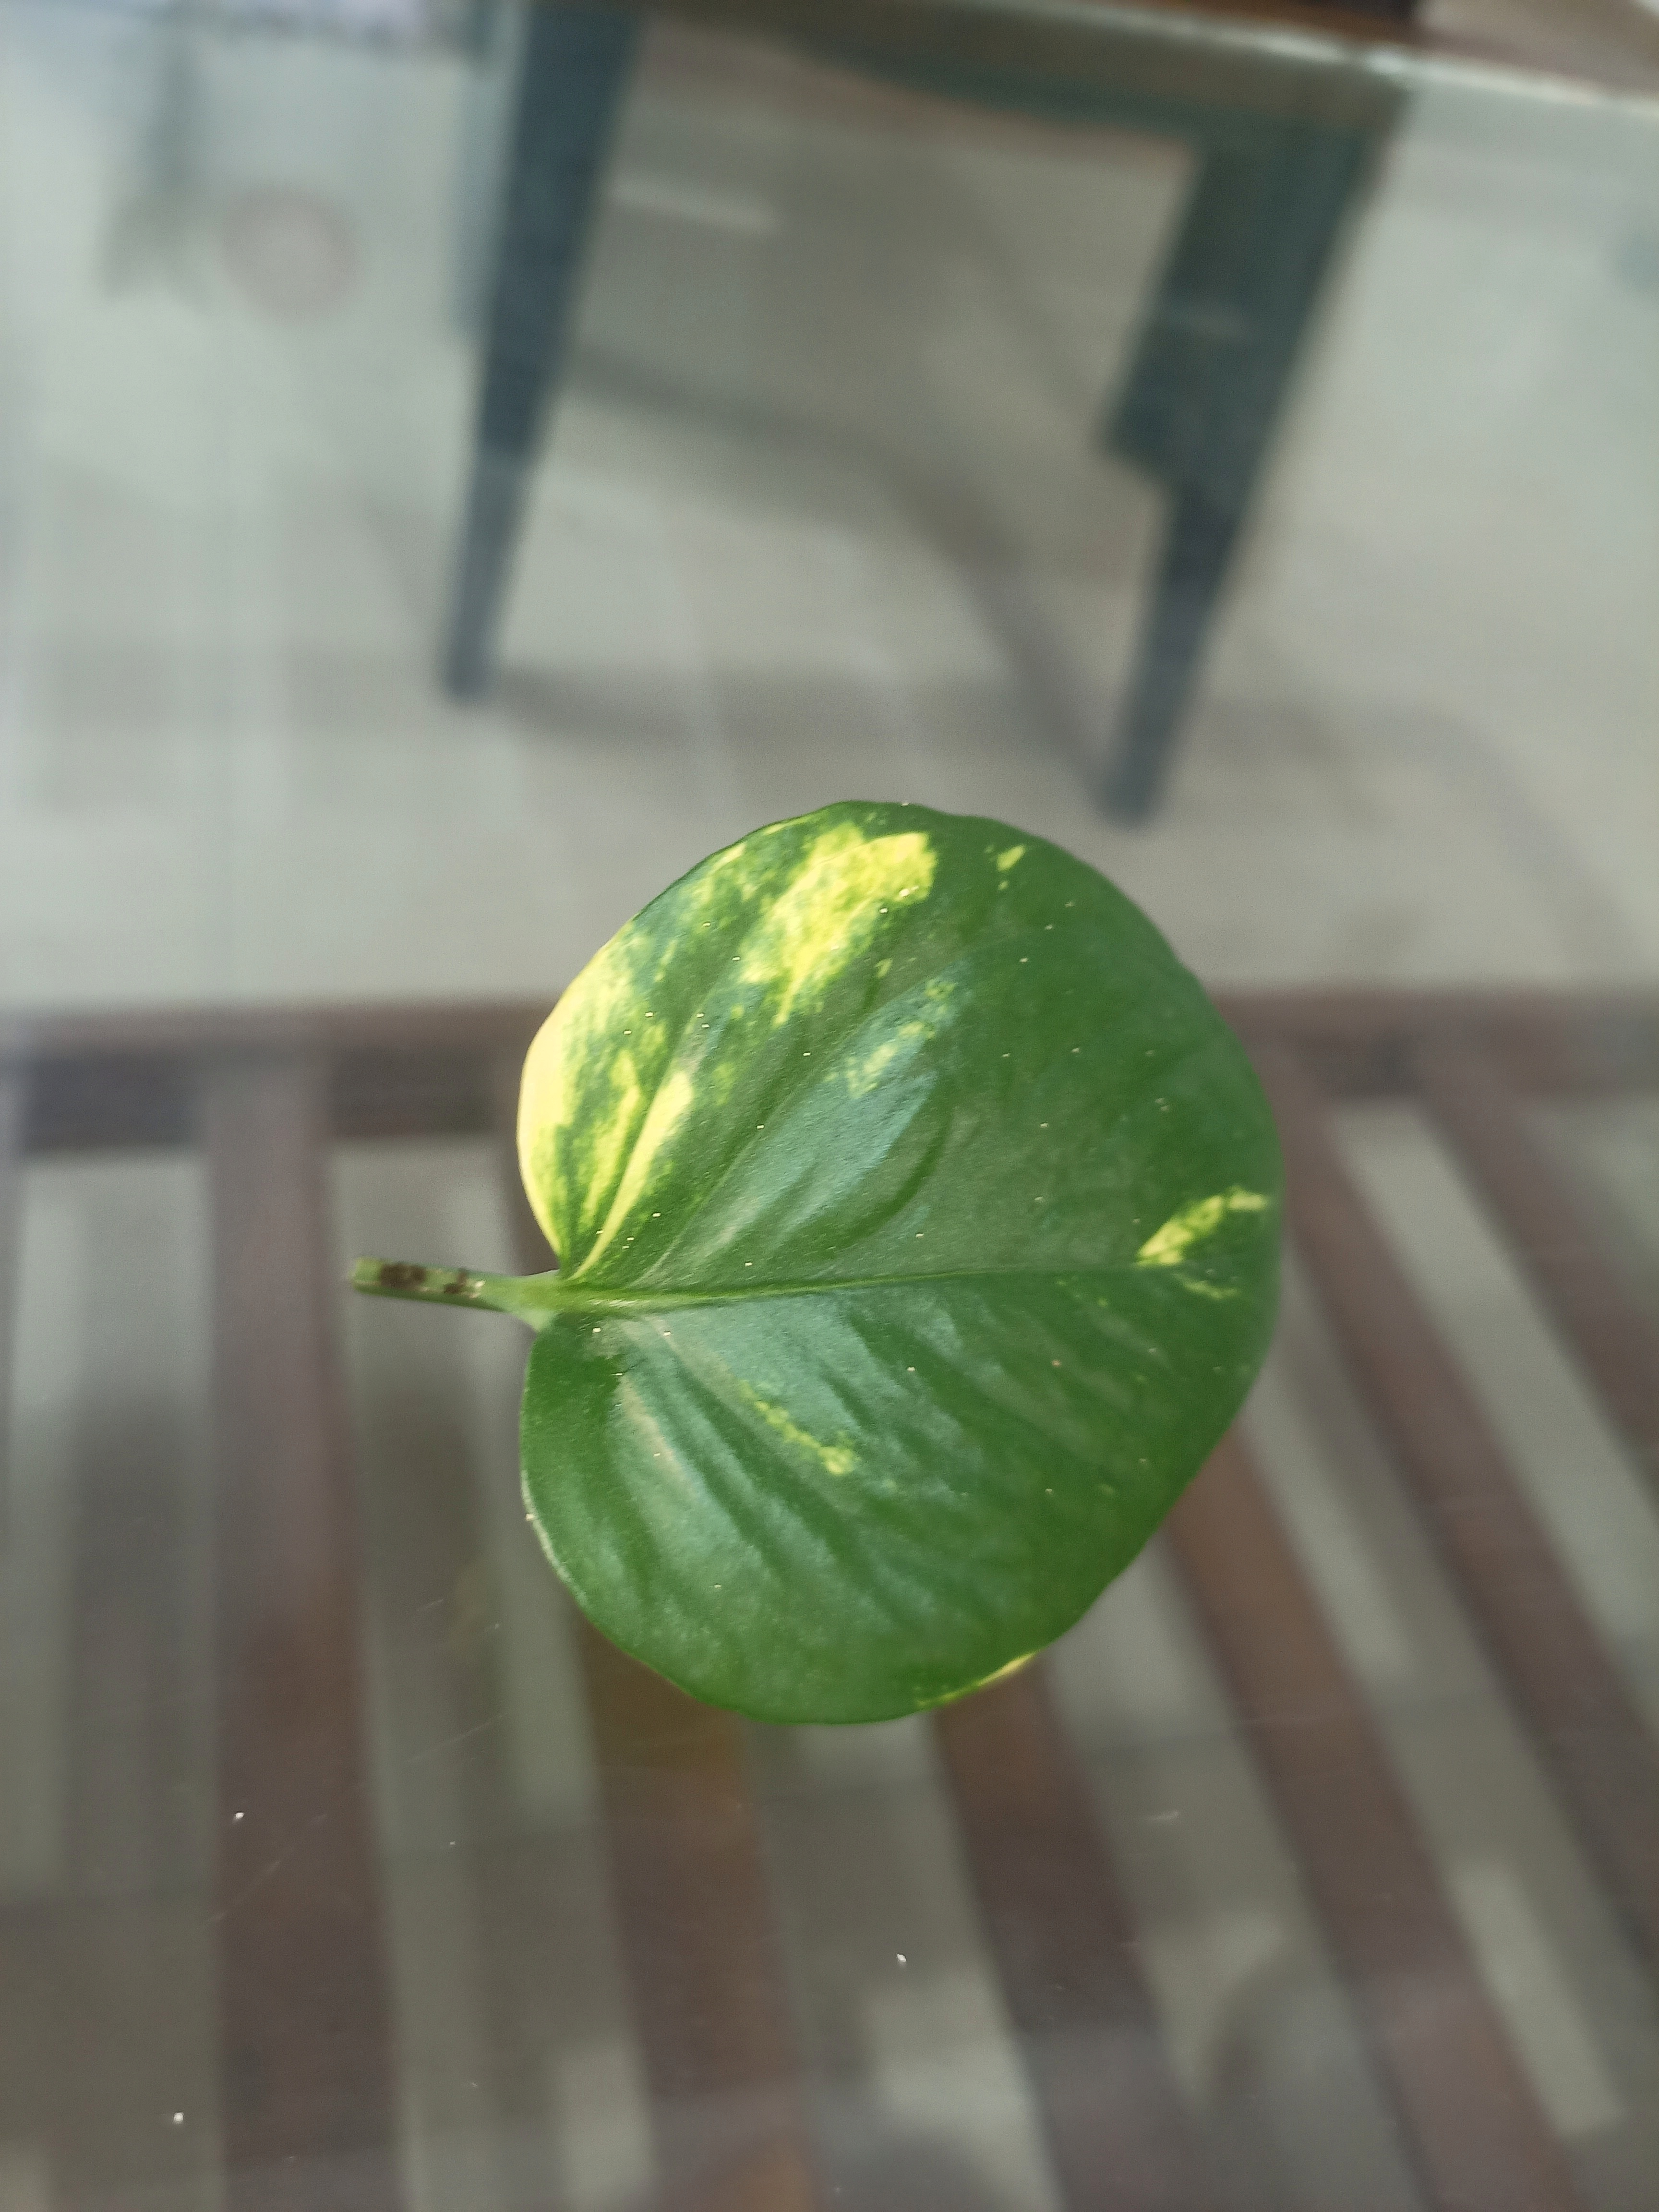
\includegraphics[width=\textwidth]{money2}
    \end{subfigure}
    \hfill
    \begin{subfigure}[b]{0.30\columnwidth}
        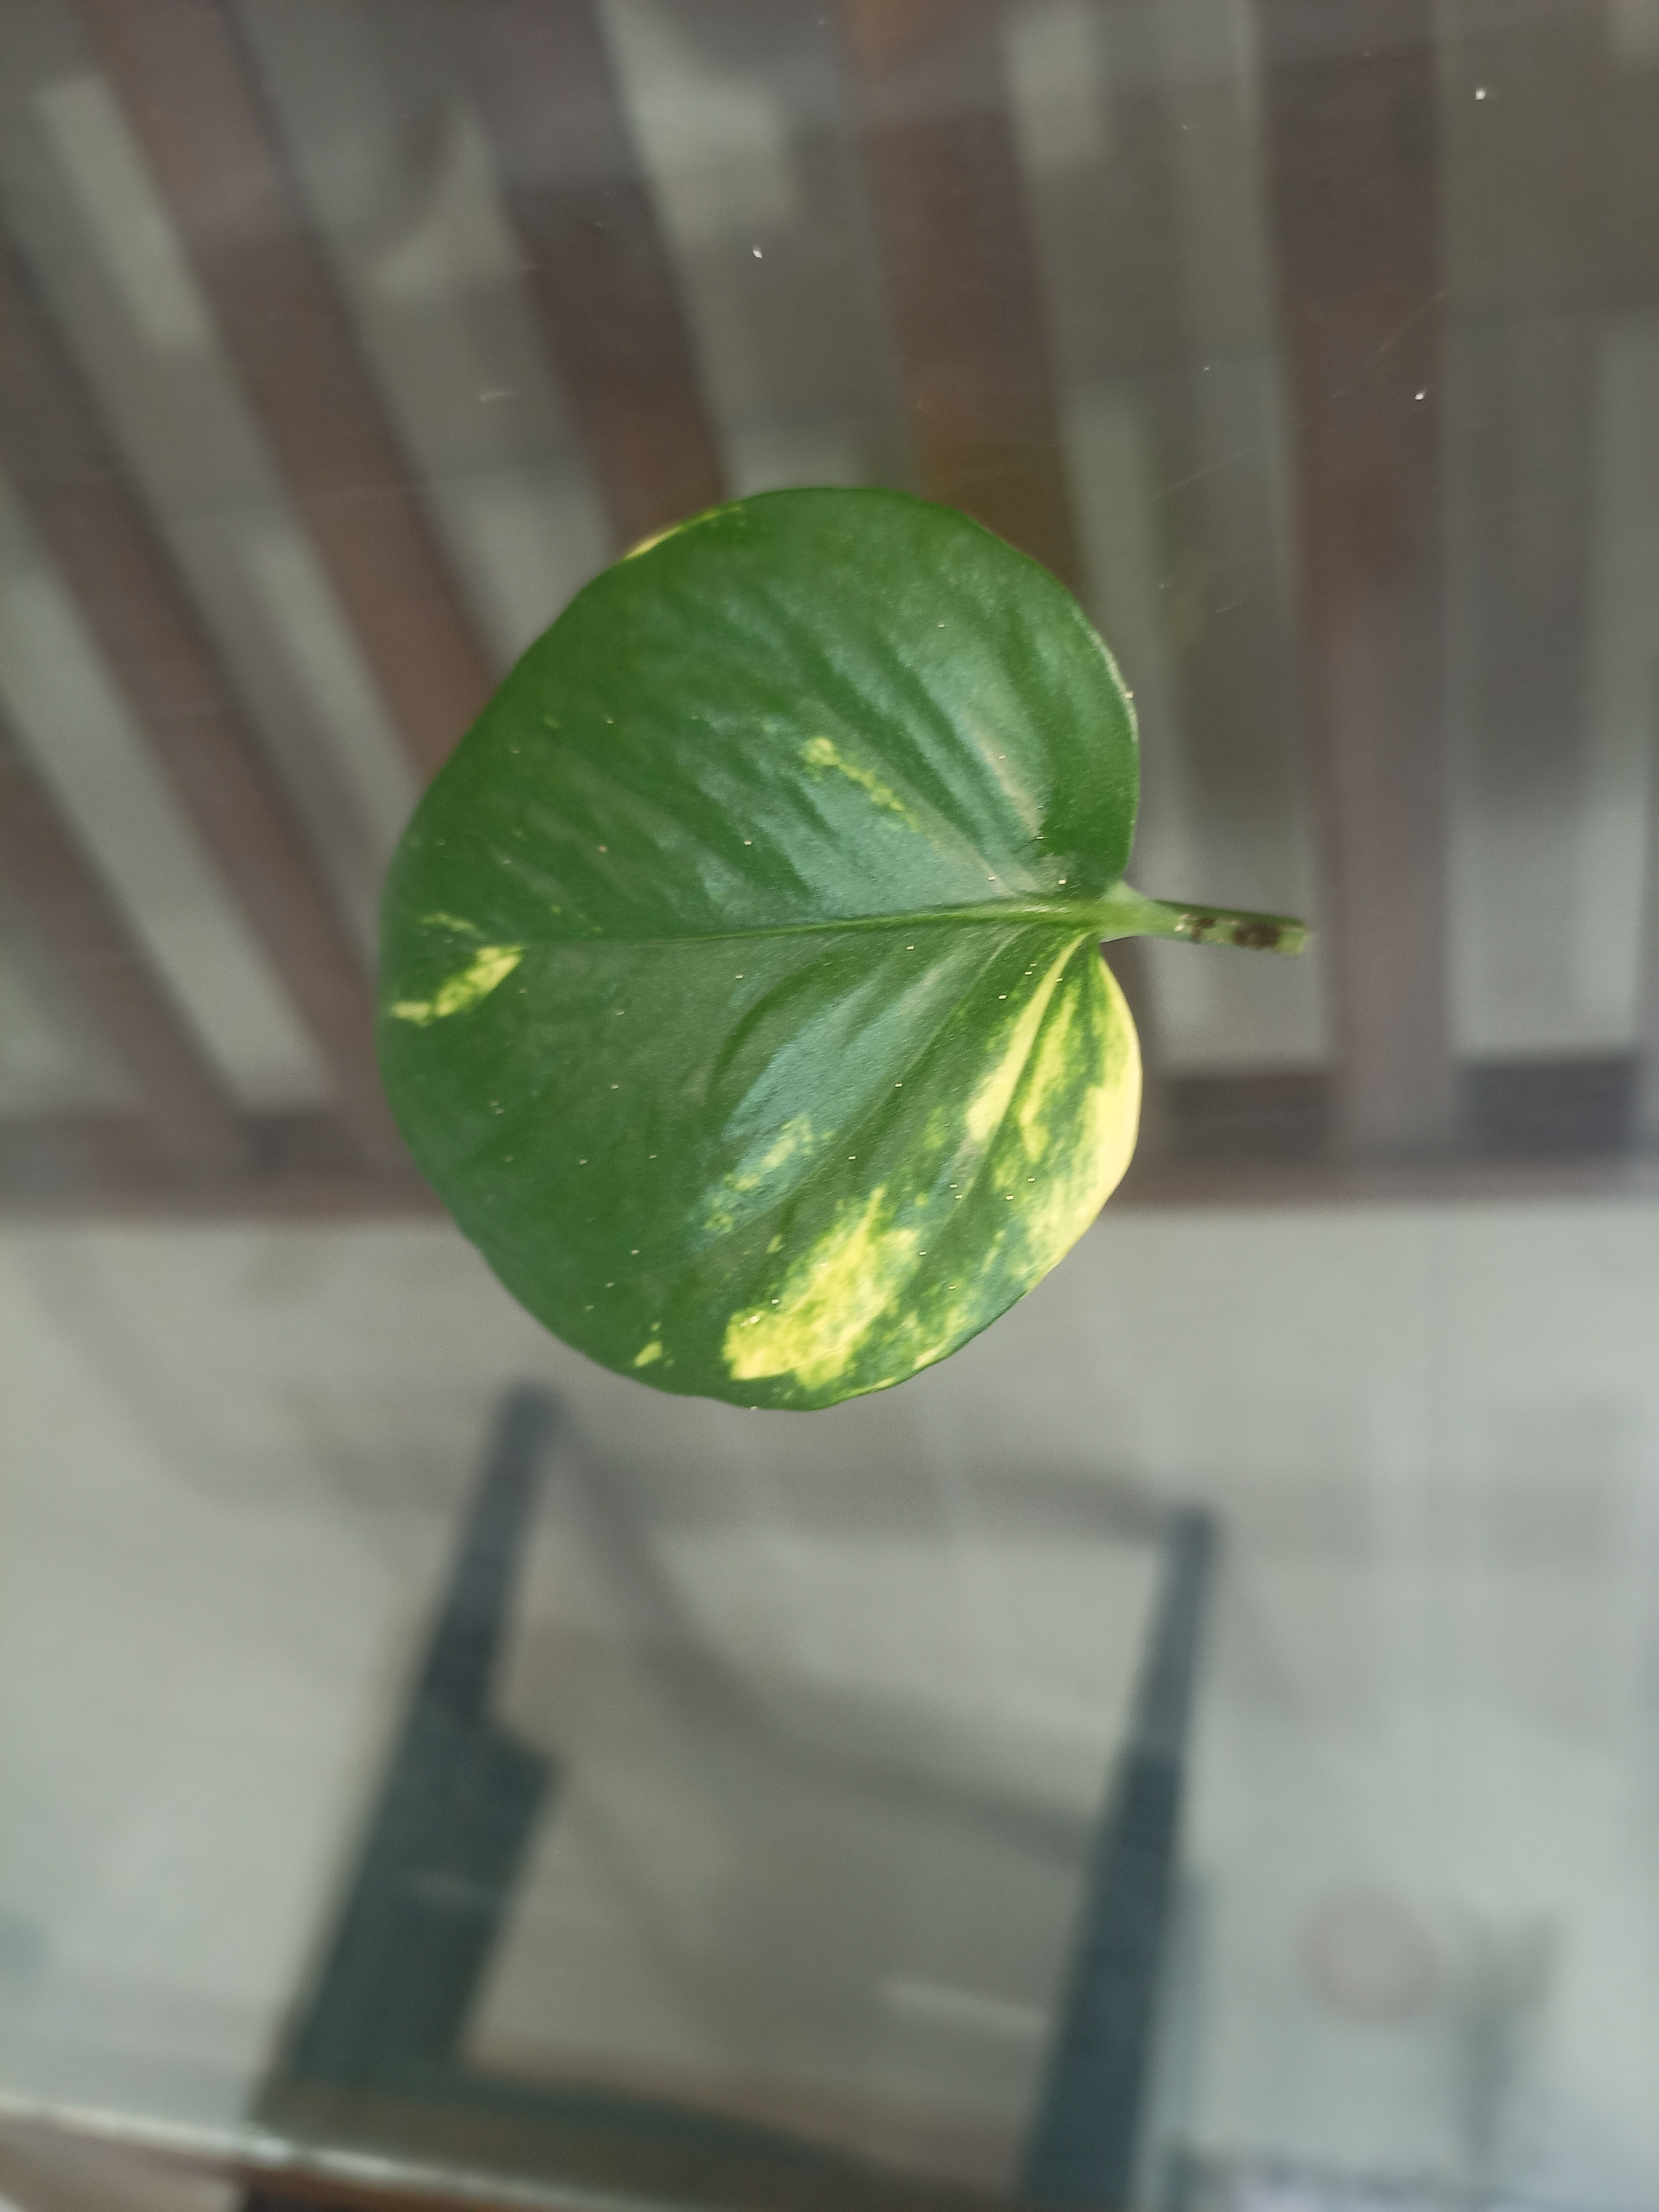
\includegraphics[width=\textwidth]{money3}
    \end{subfigure}
    \vspace{0.5em}
    
    \begin{subfigure}[b]{0.30\columnwidth}
        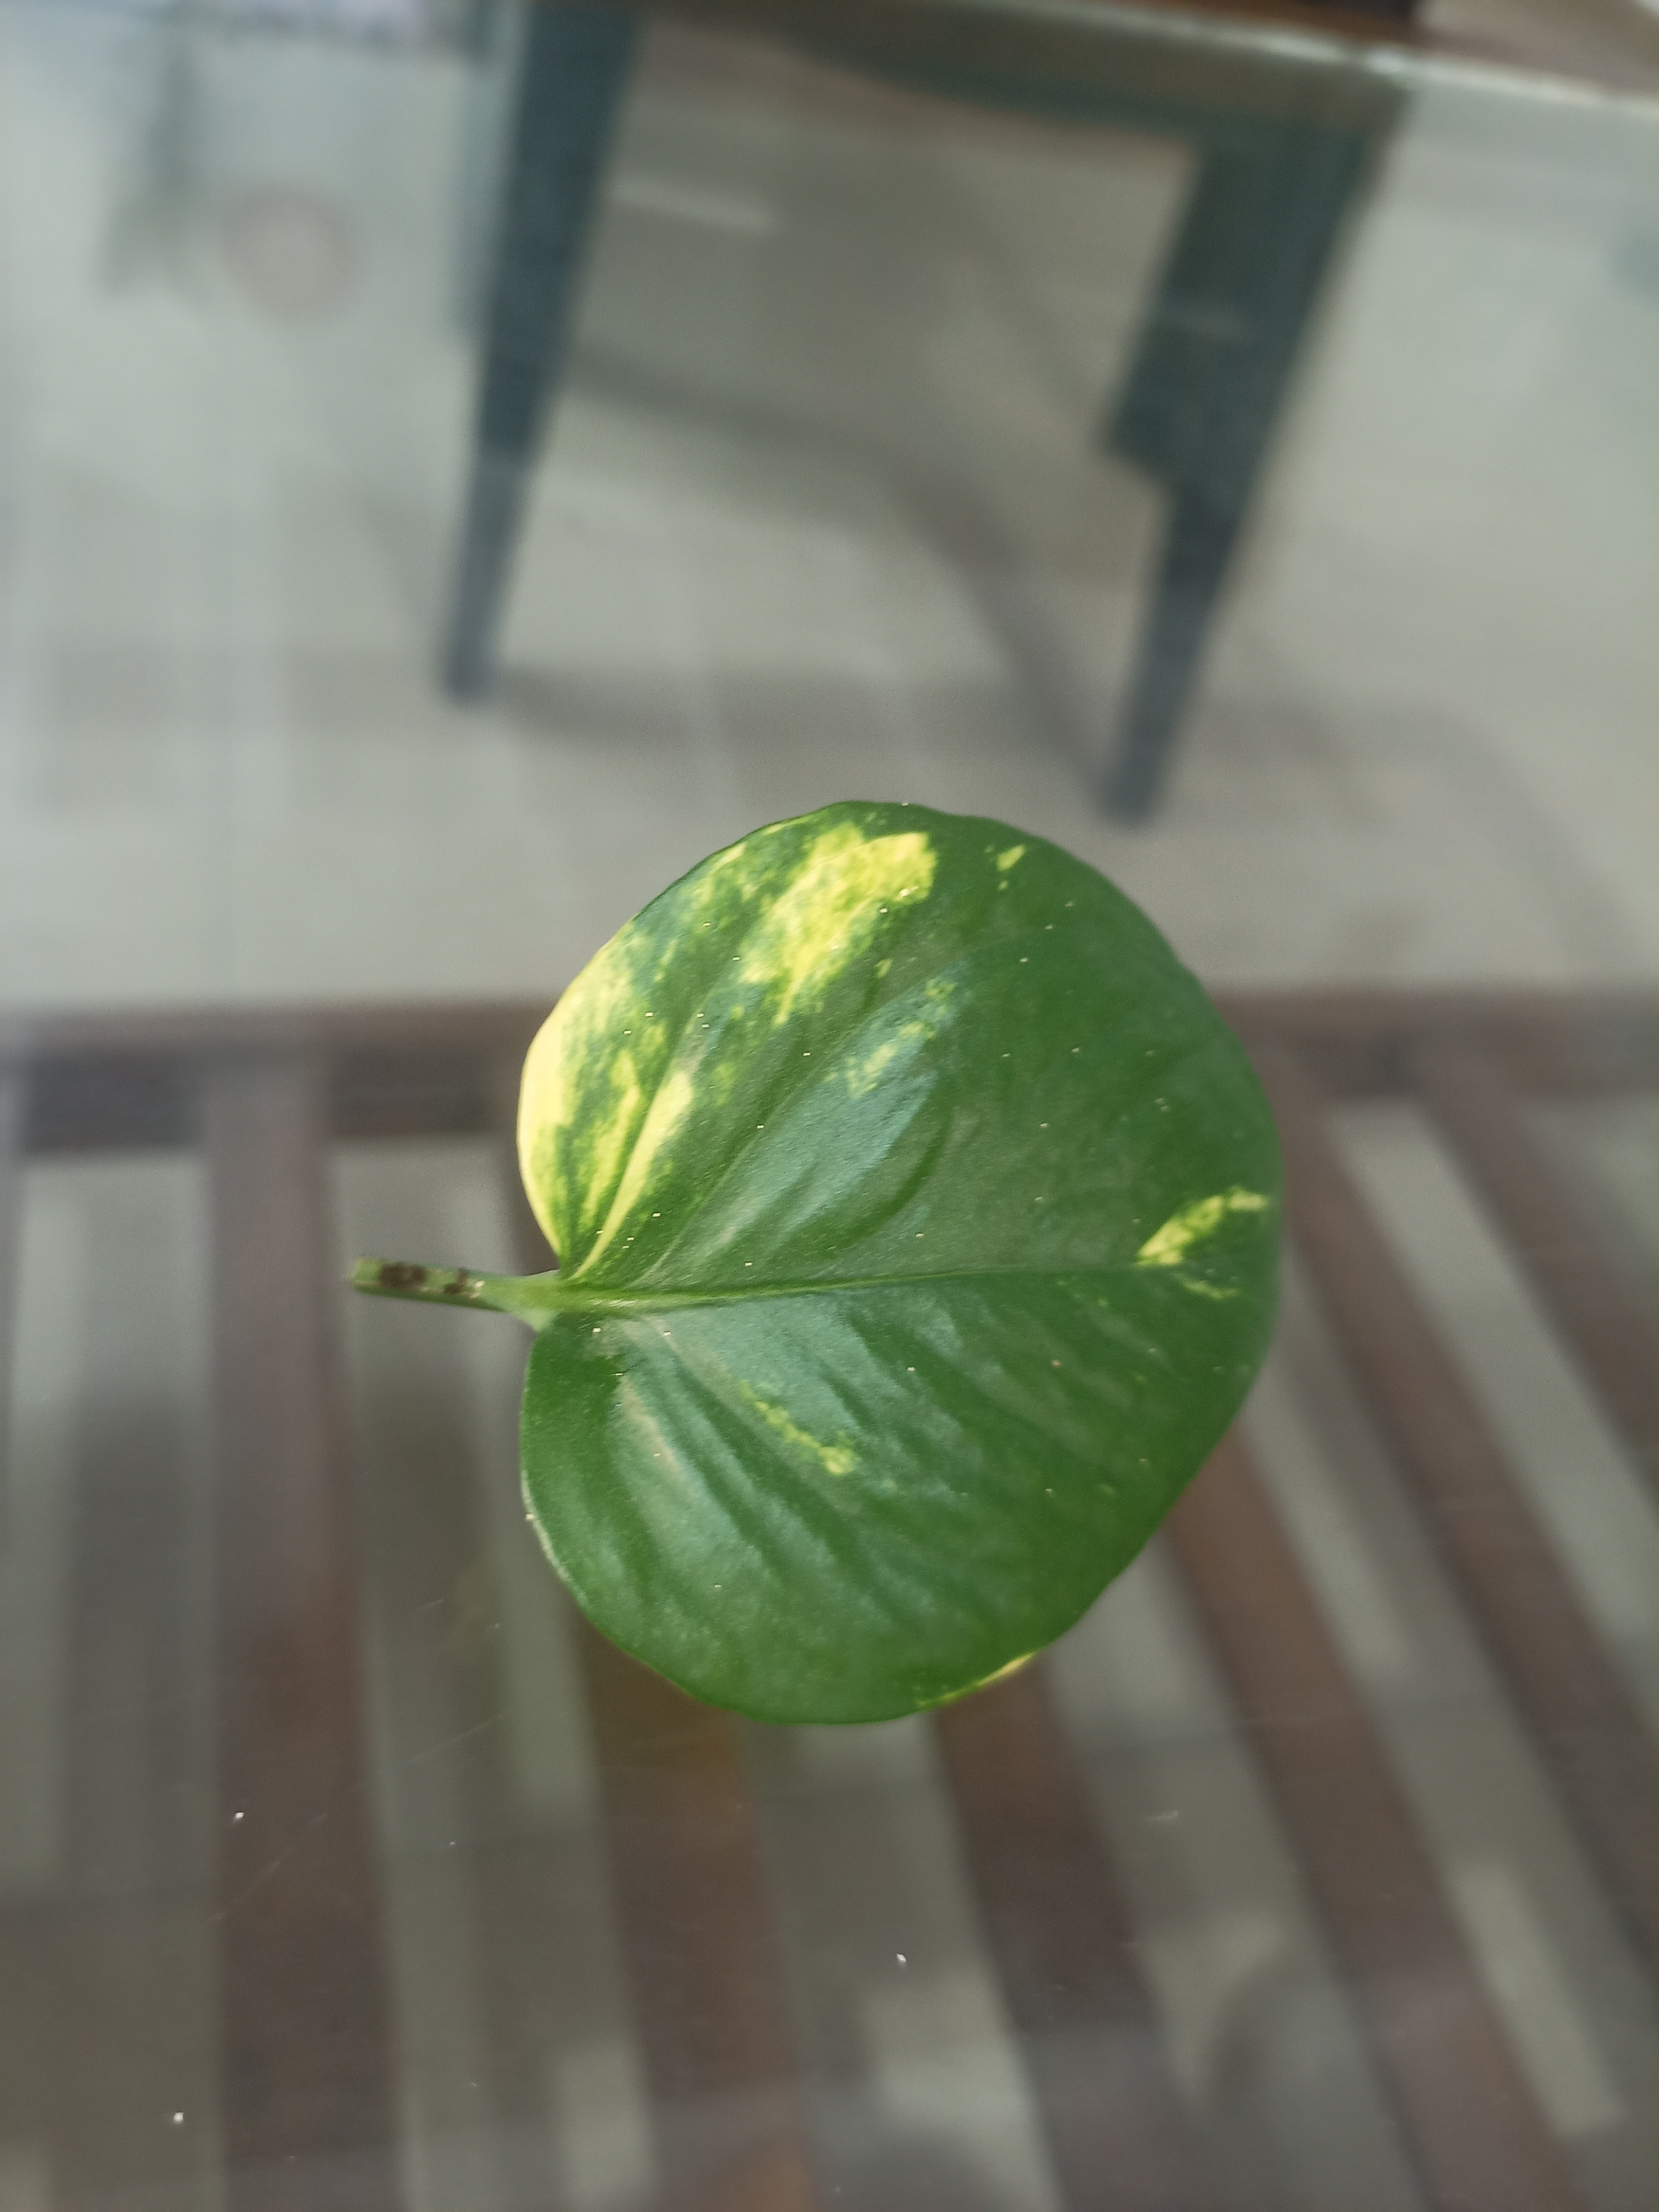
\includegraphics[width=\textwidth]{money4}
    \end{subfigure}
    \hfill
    \begin{subfigure}[b]{0.30\columnwidth}
        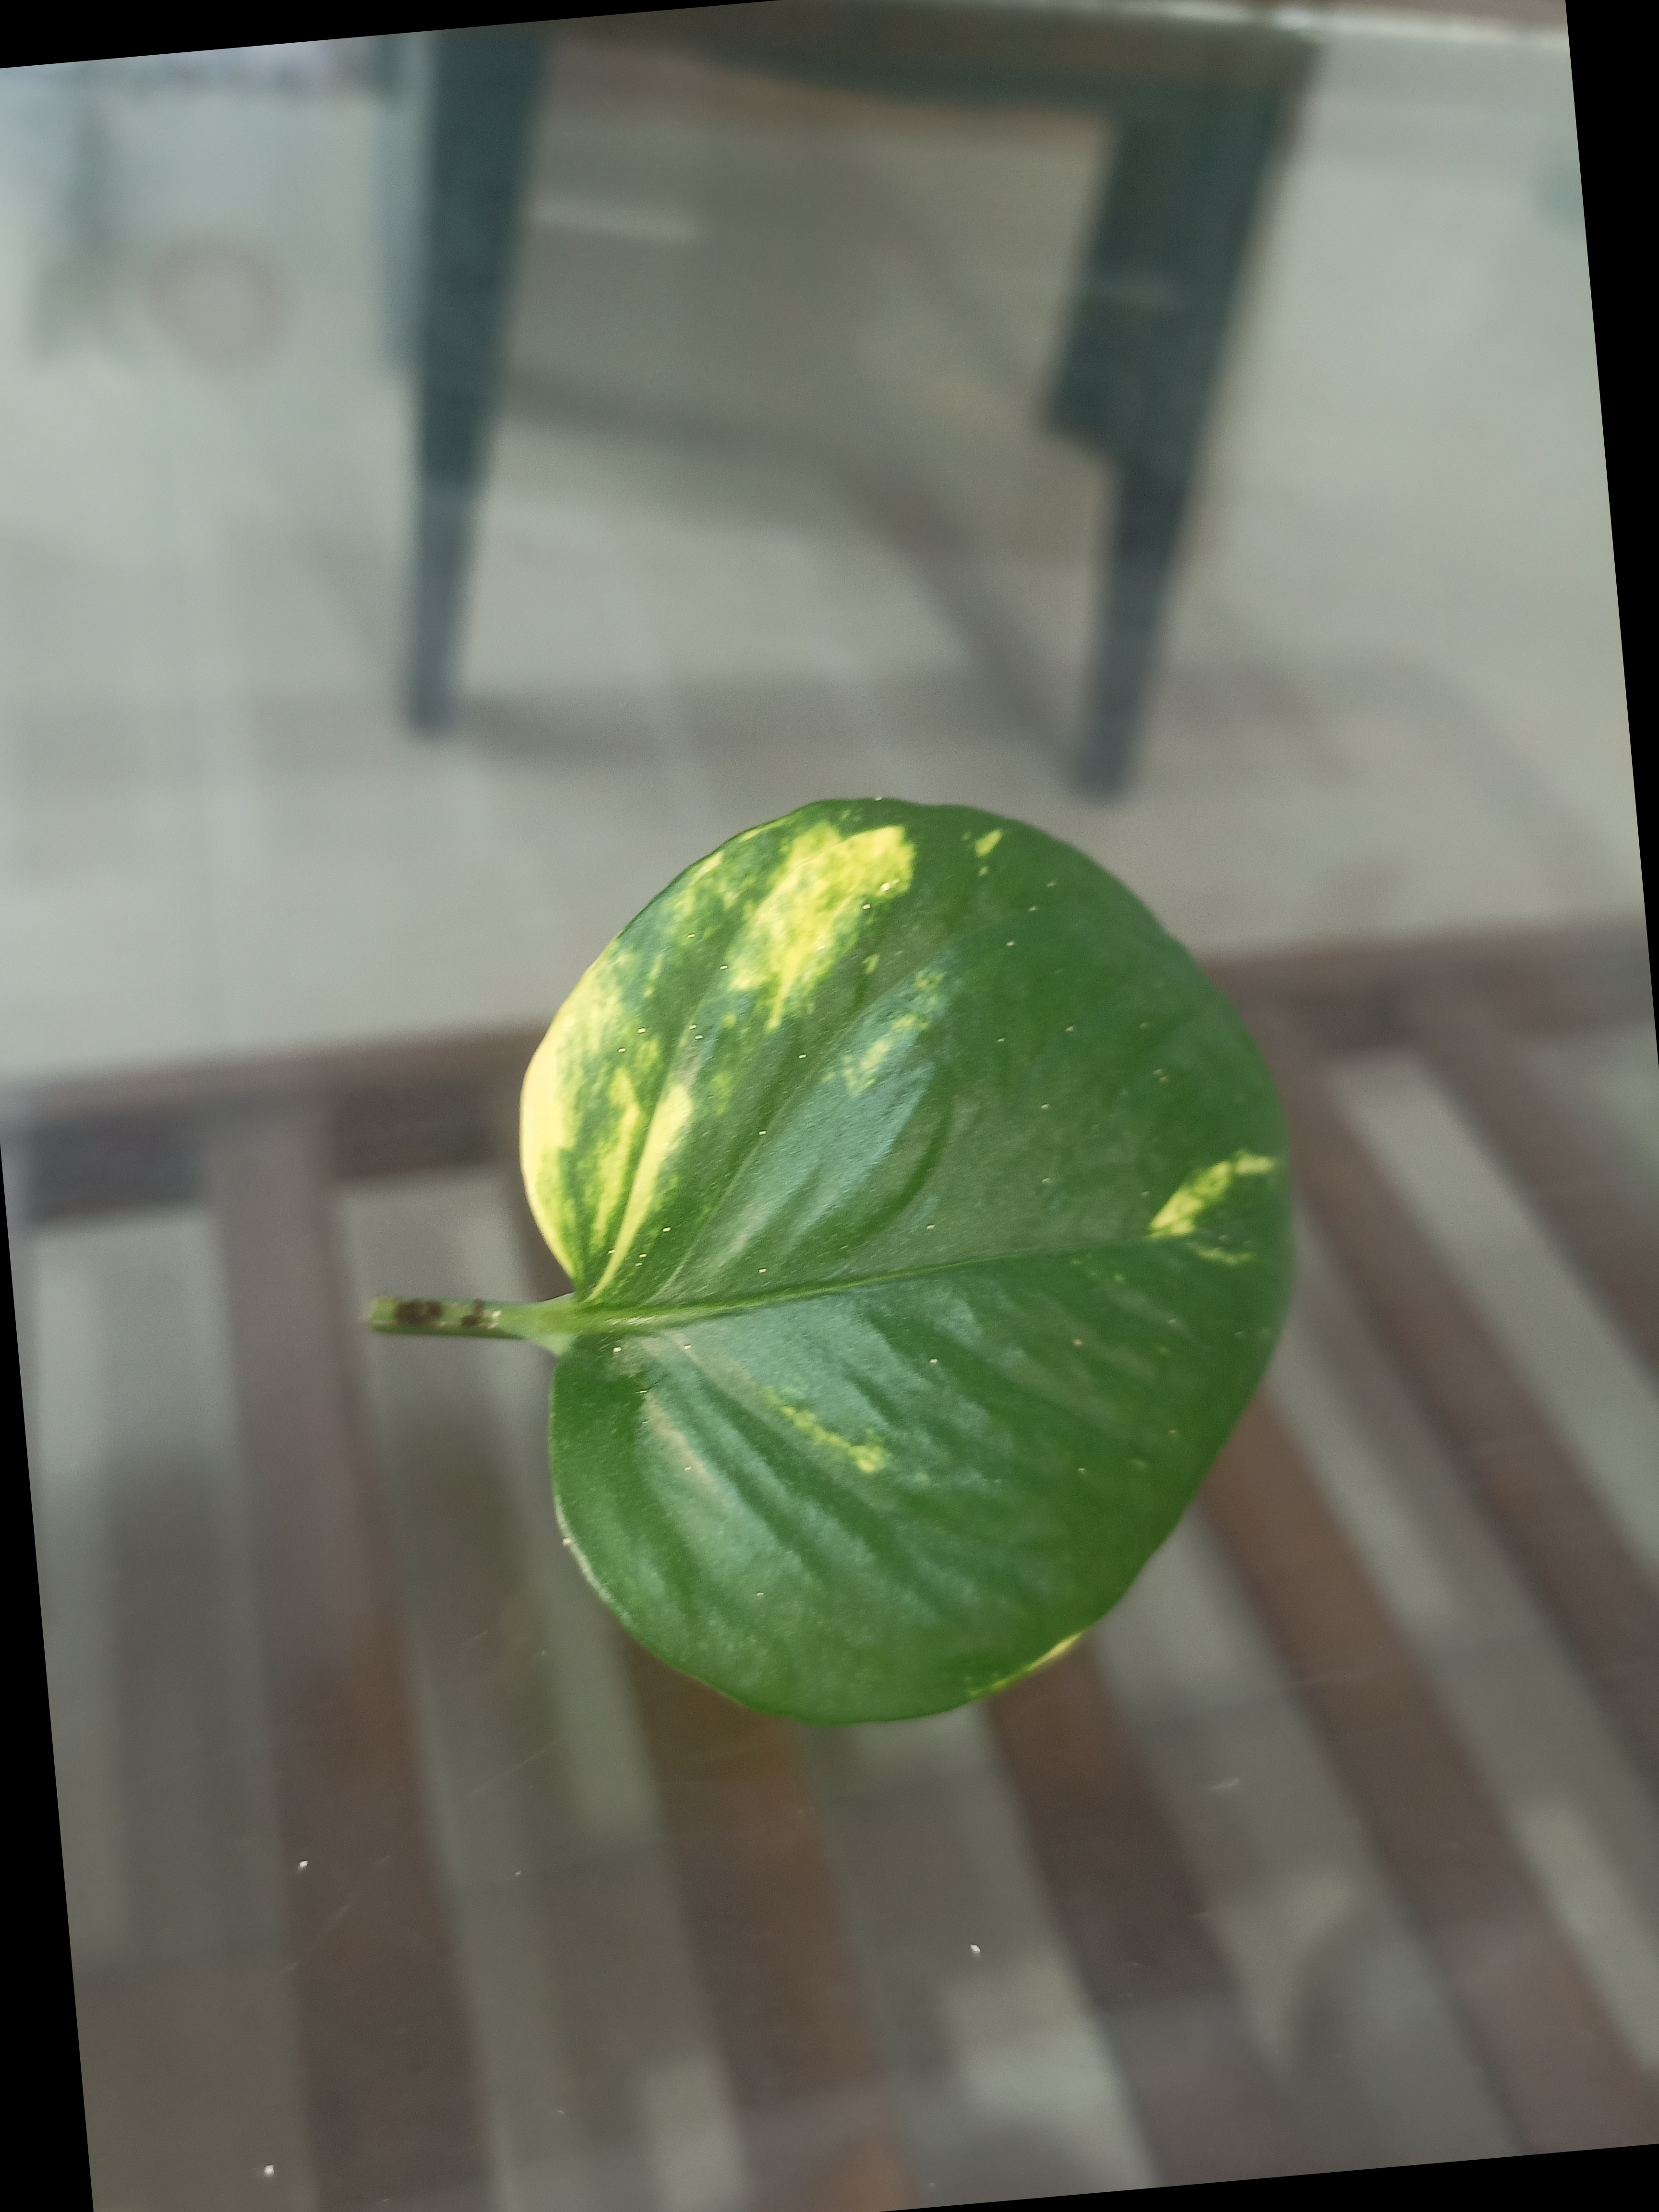
\includegraphics[width=\textwidth]{money5}
    \end{subfigure}
    \hfill
    \begin{subfigure}[b]{0.30\columnwidth}
        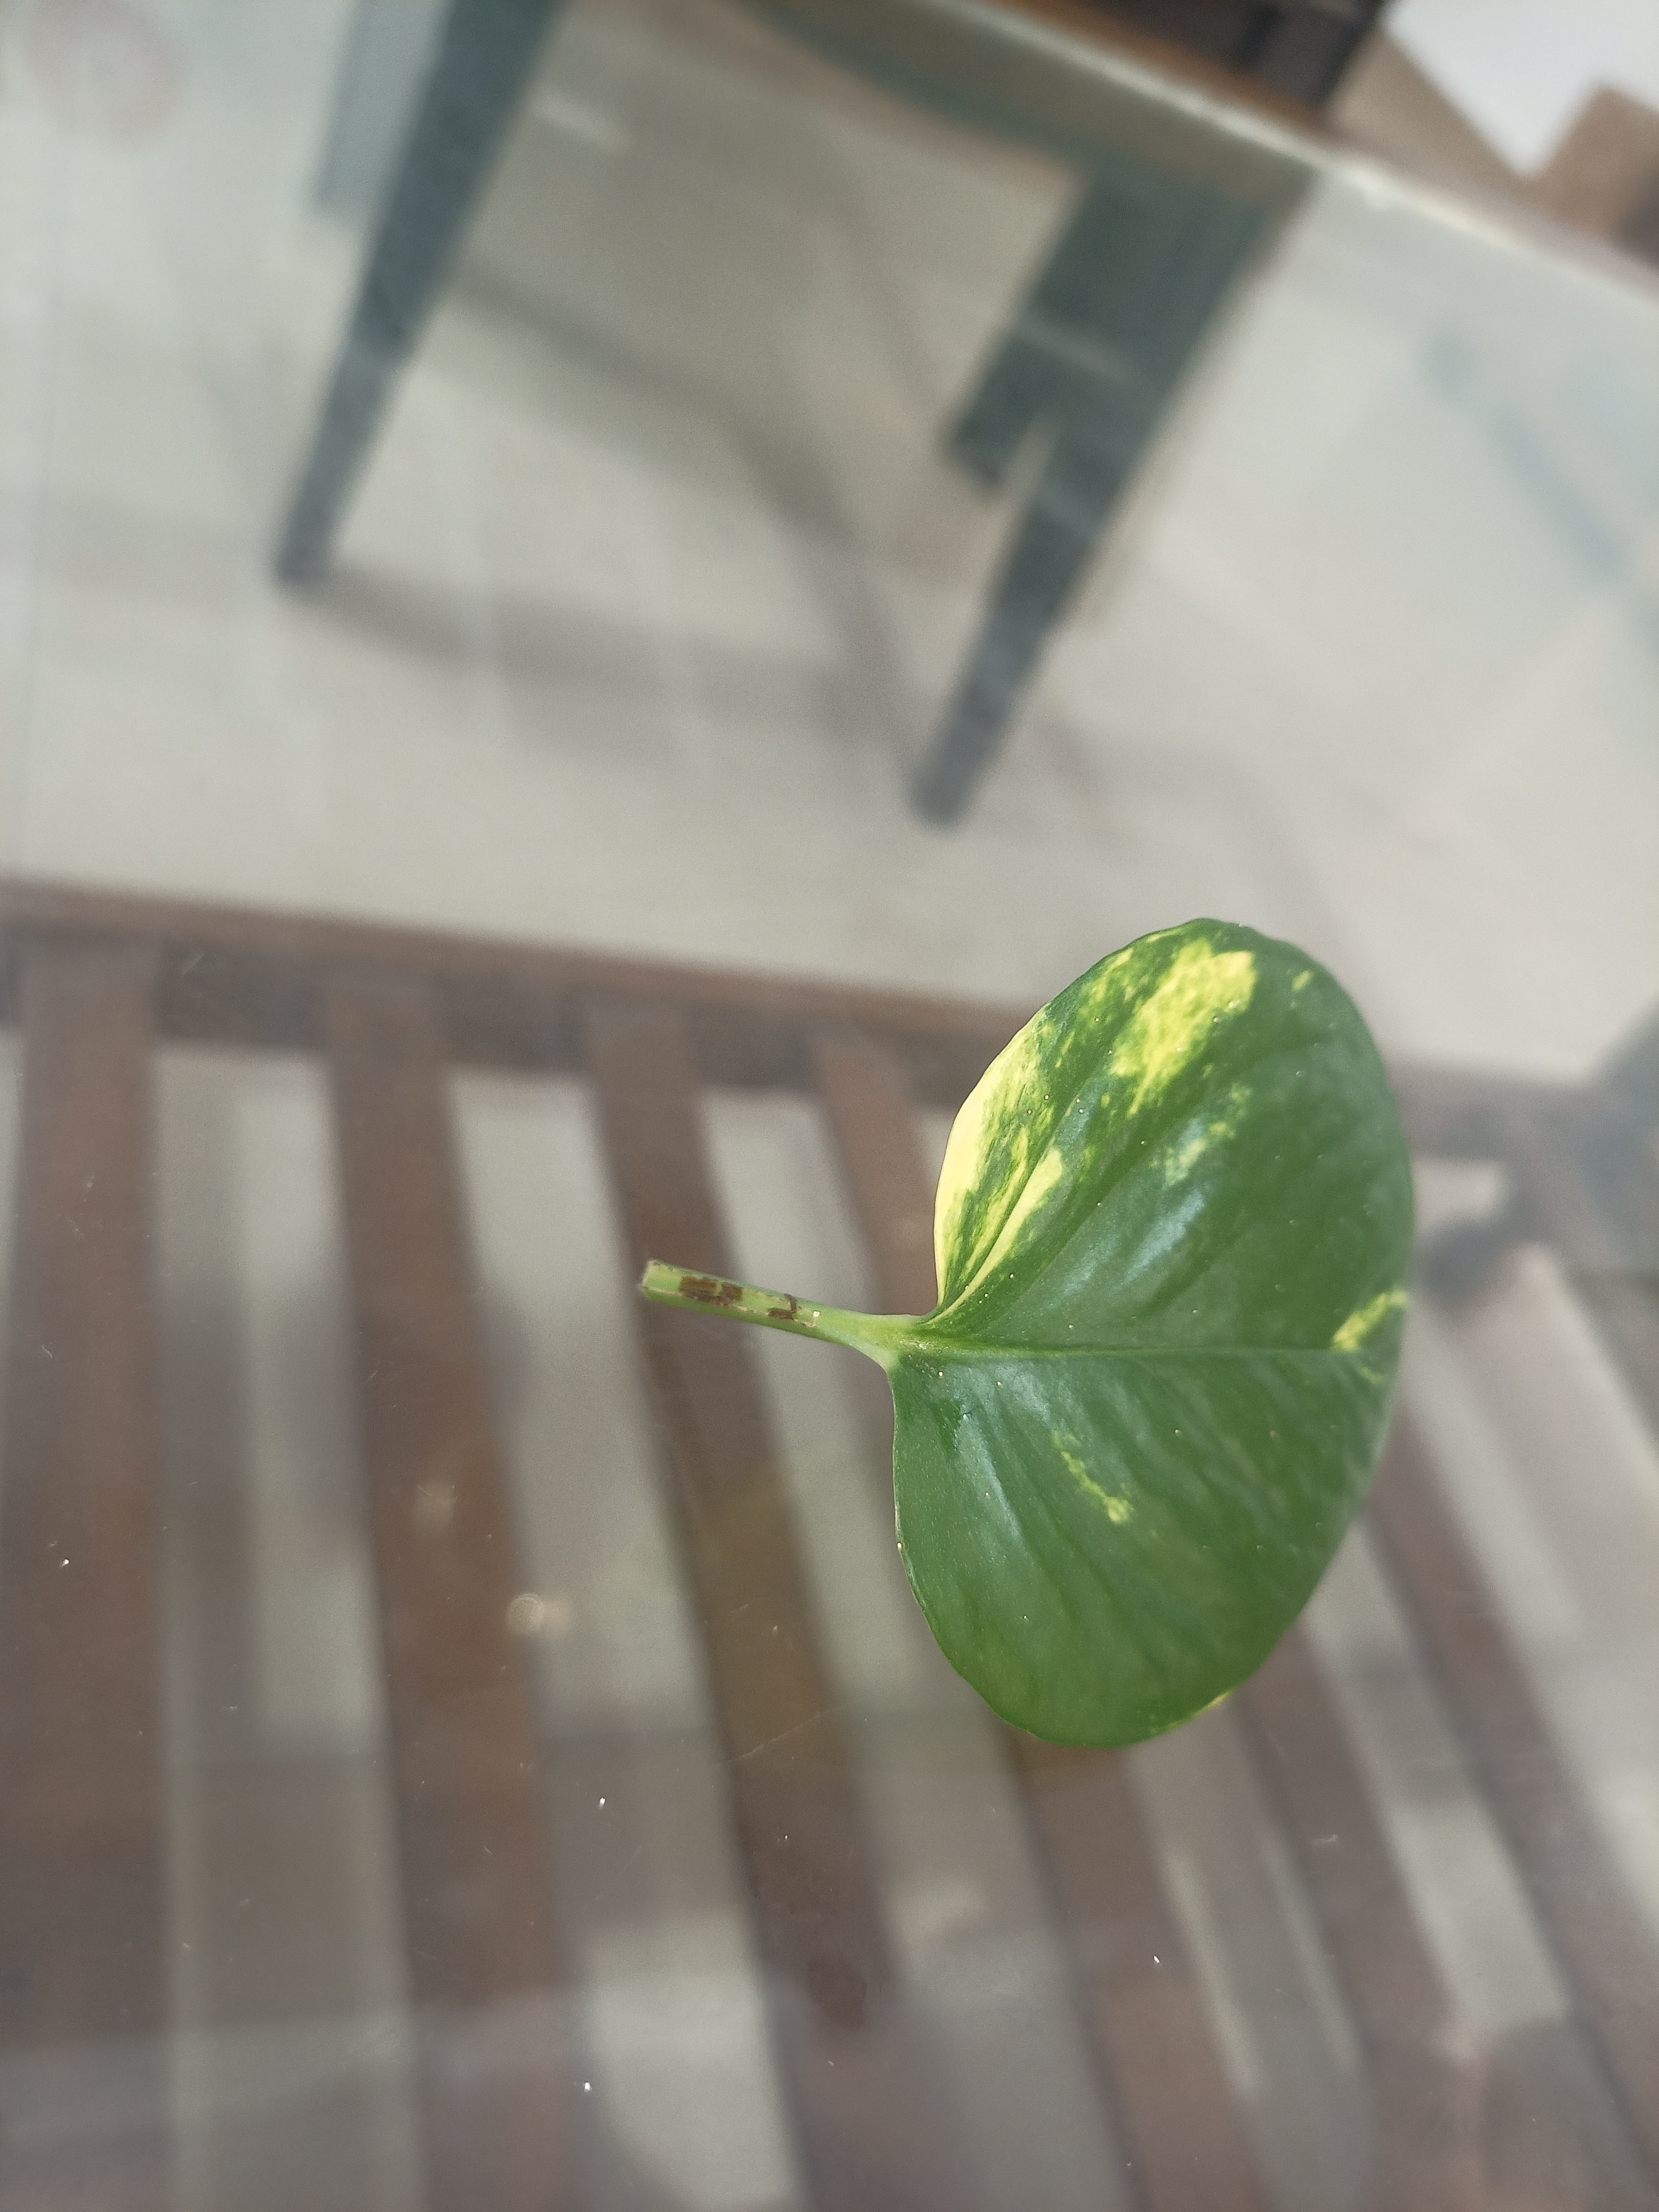
\includegraphics[width=\textwidth]{money6}
    \end{subfigure}
    \vspace{0.5em}
    
    \begin{subfigure}[b]{0.30\columnwidth}
        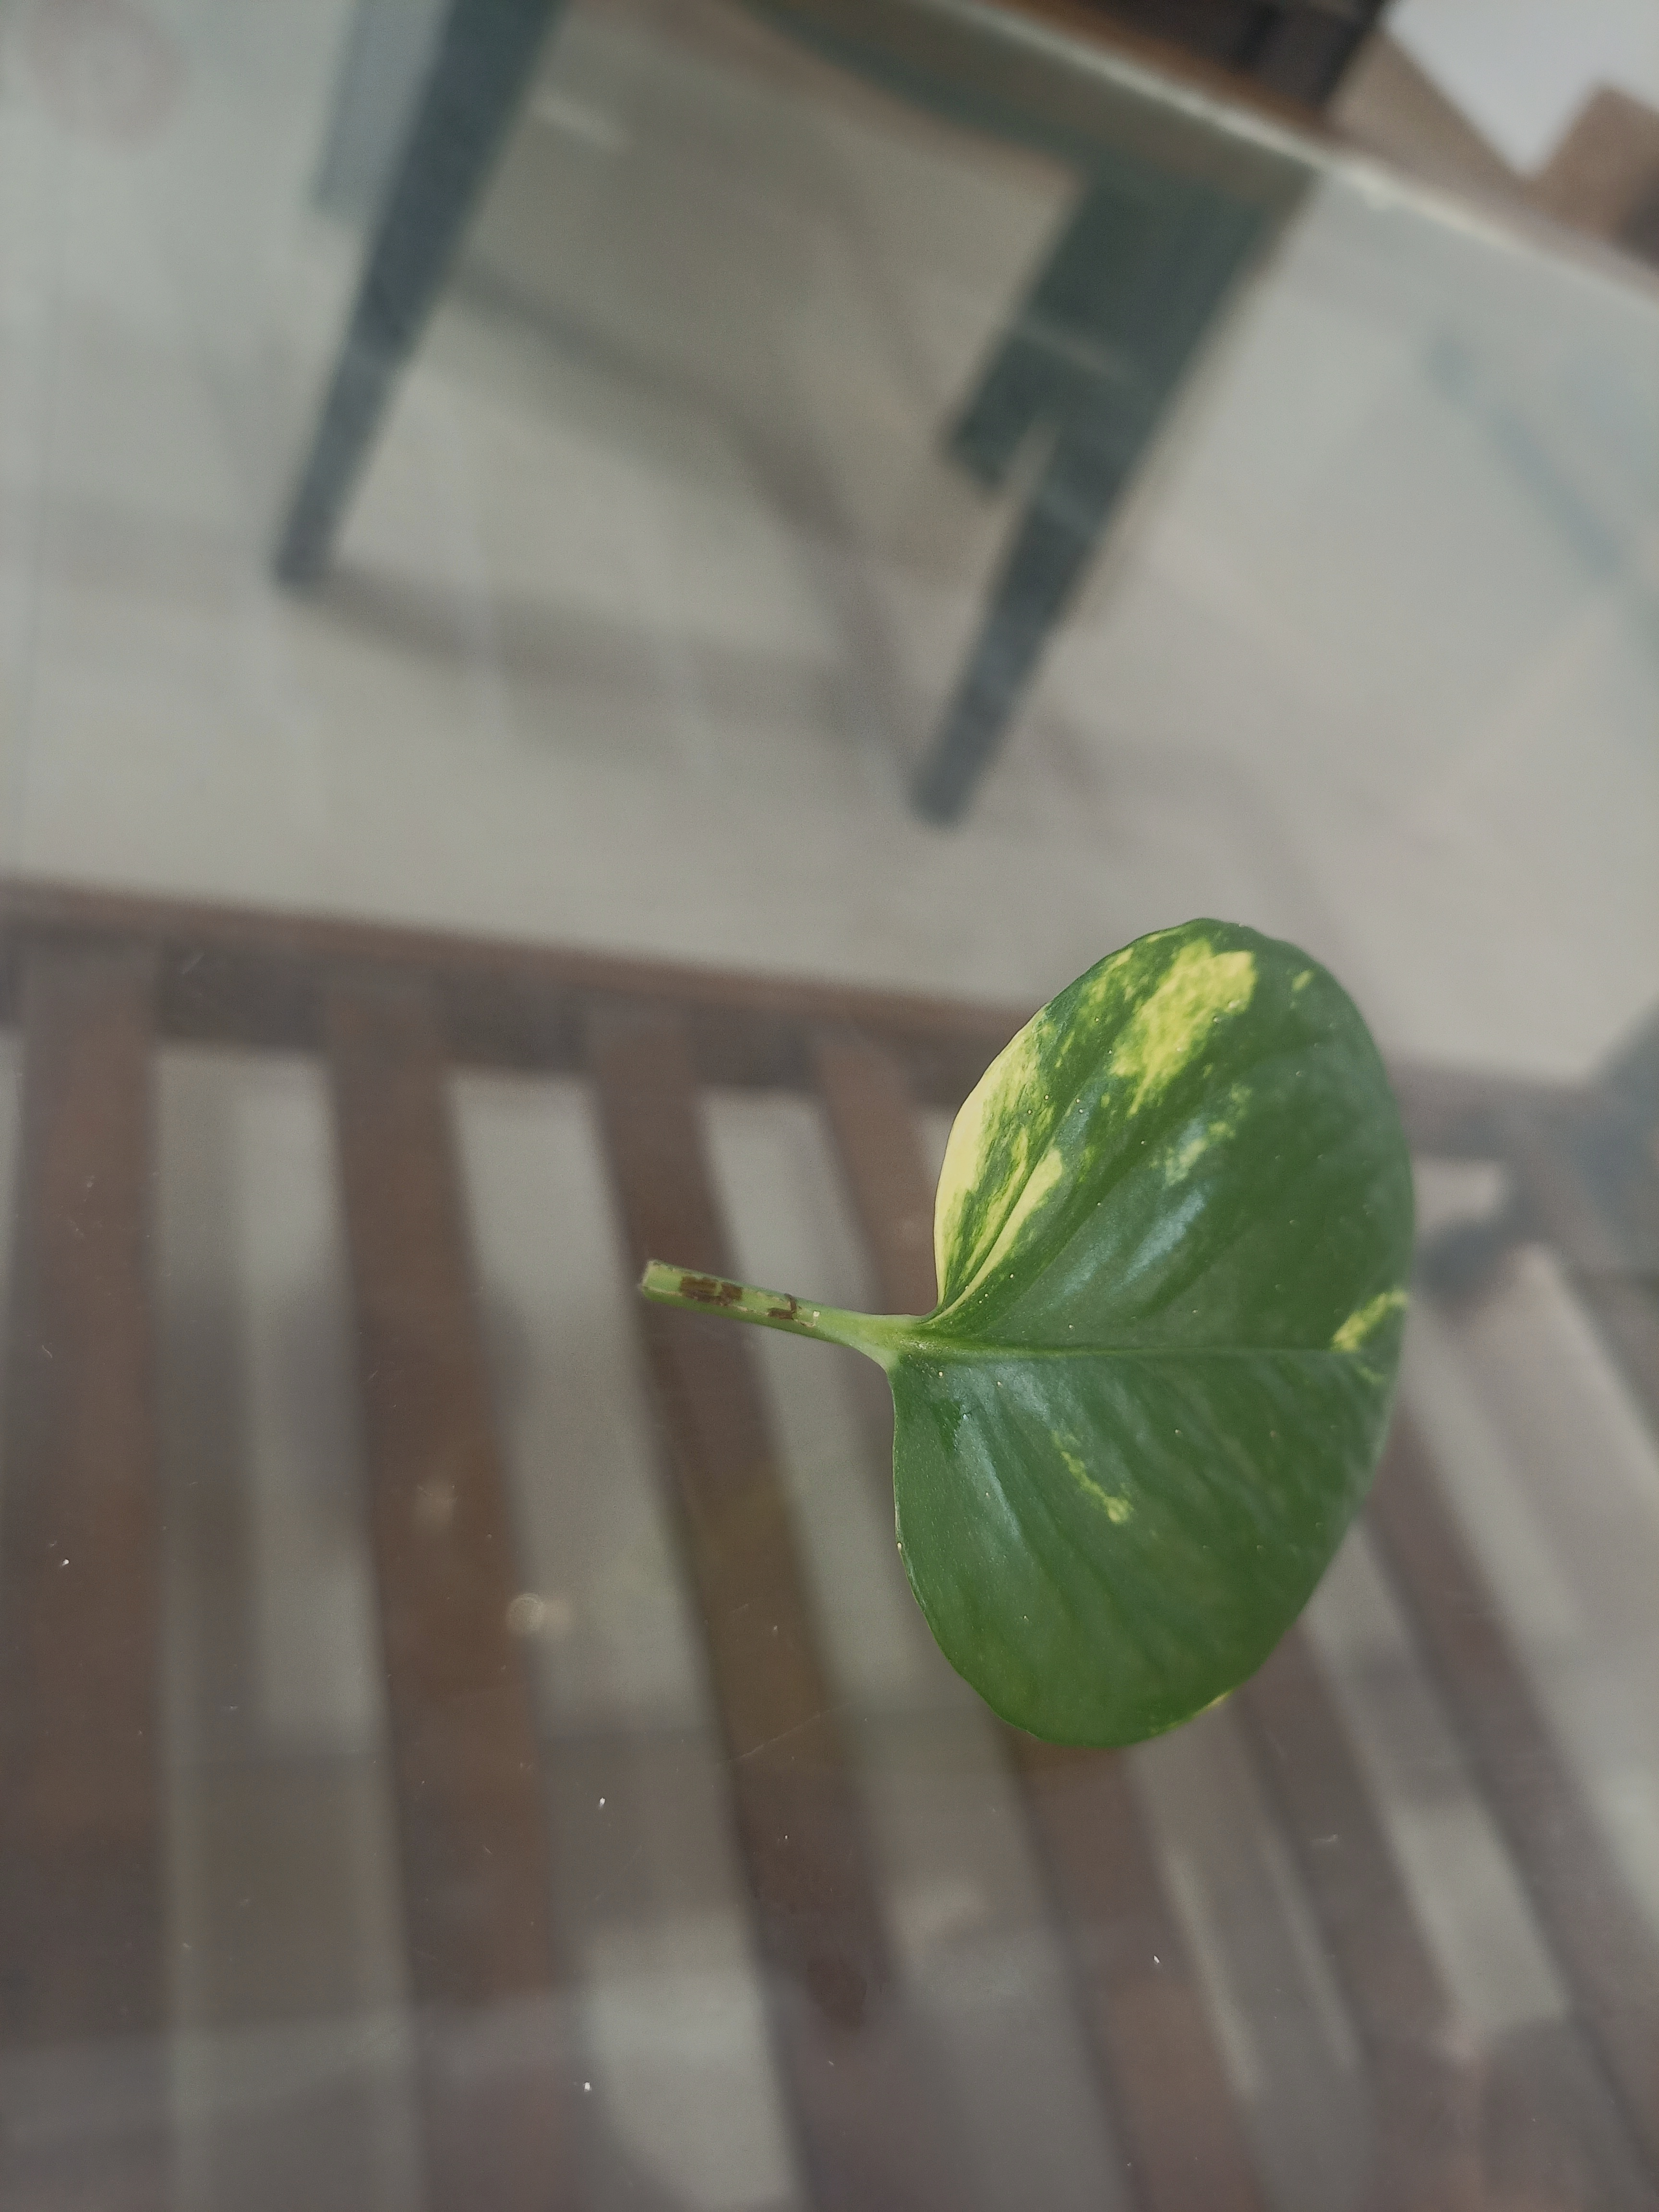
\includegraphics[width=\textwidth]{money7}
    \end{subfigure}
    \hfill
    \begin{subfigure}[b]{0.30\columnwidth}
        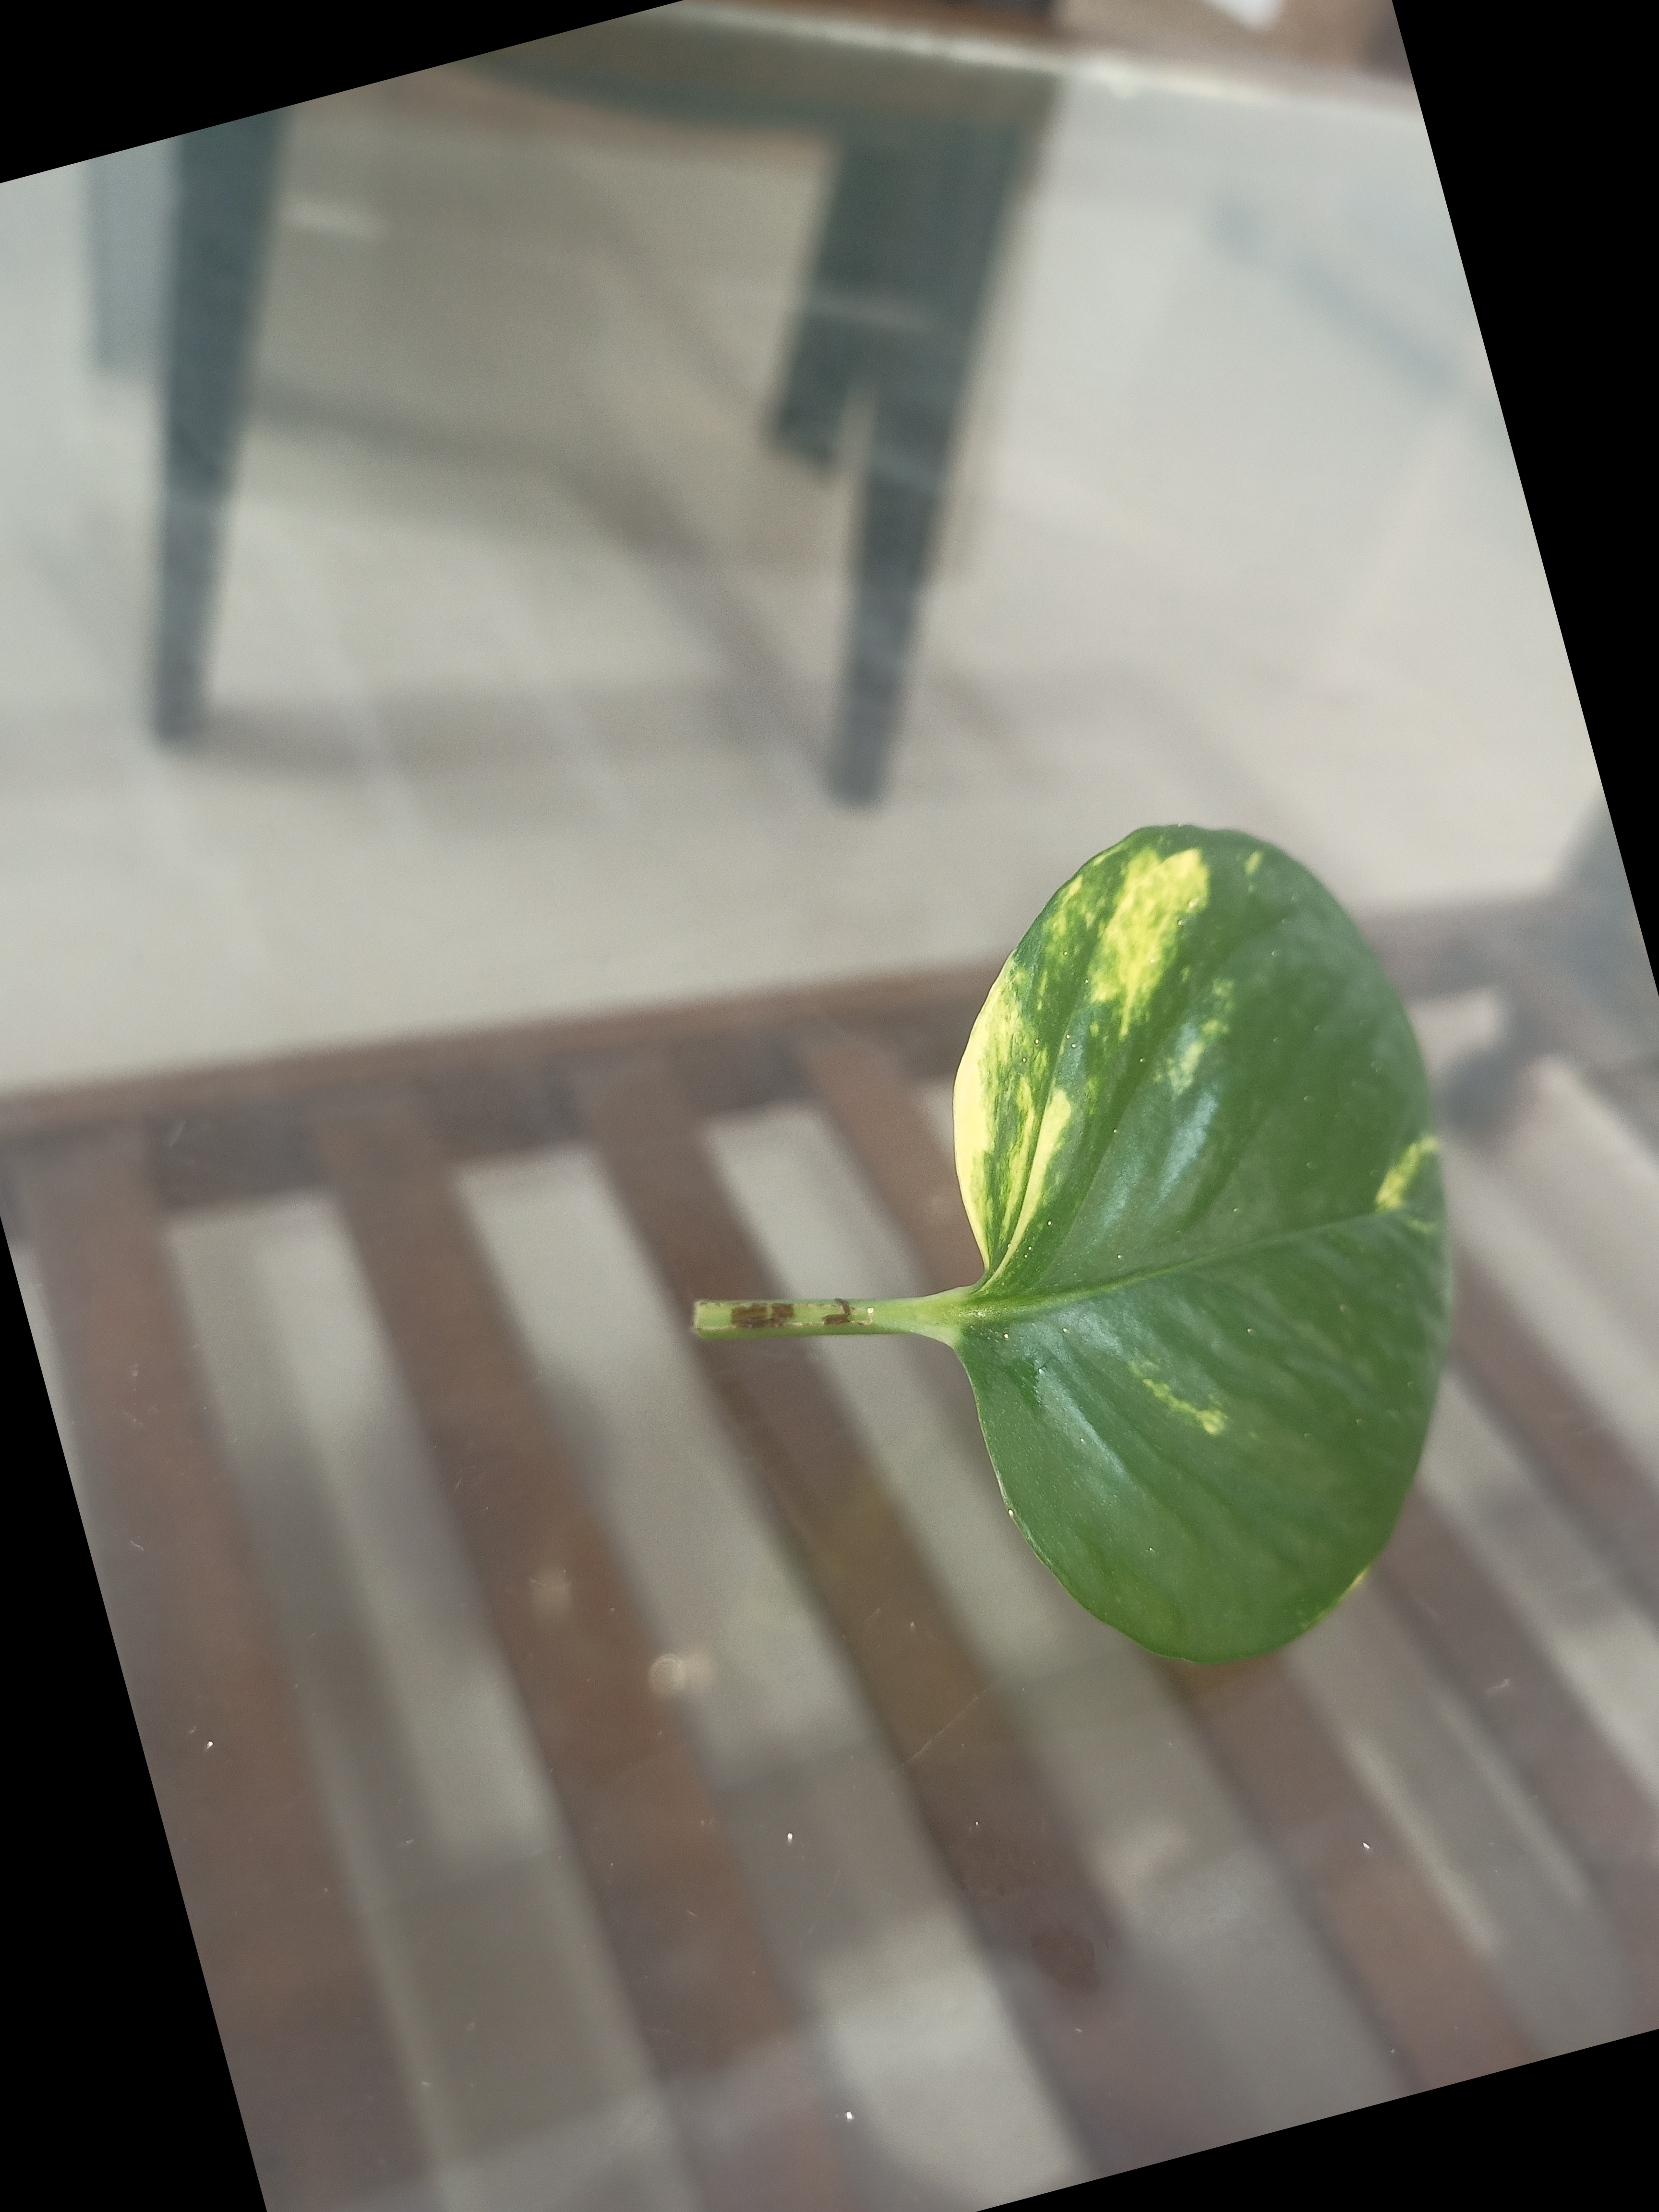
\includegraphics[width=\textwidth]{money8}
    \end{subfigure}
    \hfill
    \begin{subfigure}[b]{0.30\columnwidth}
        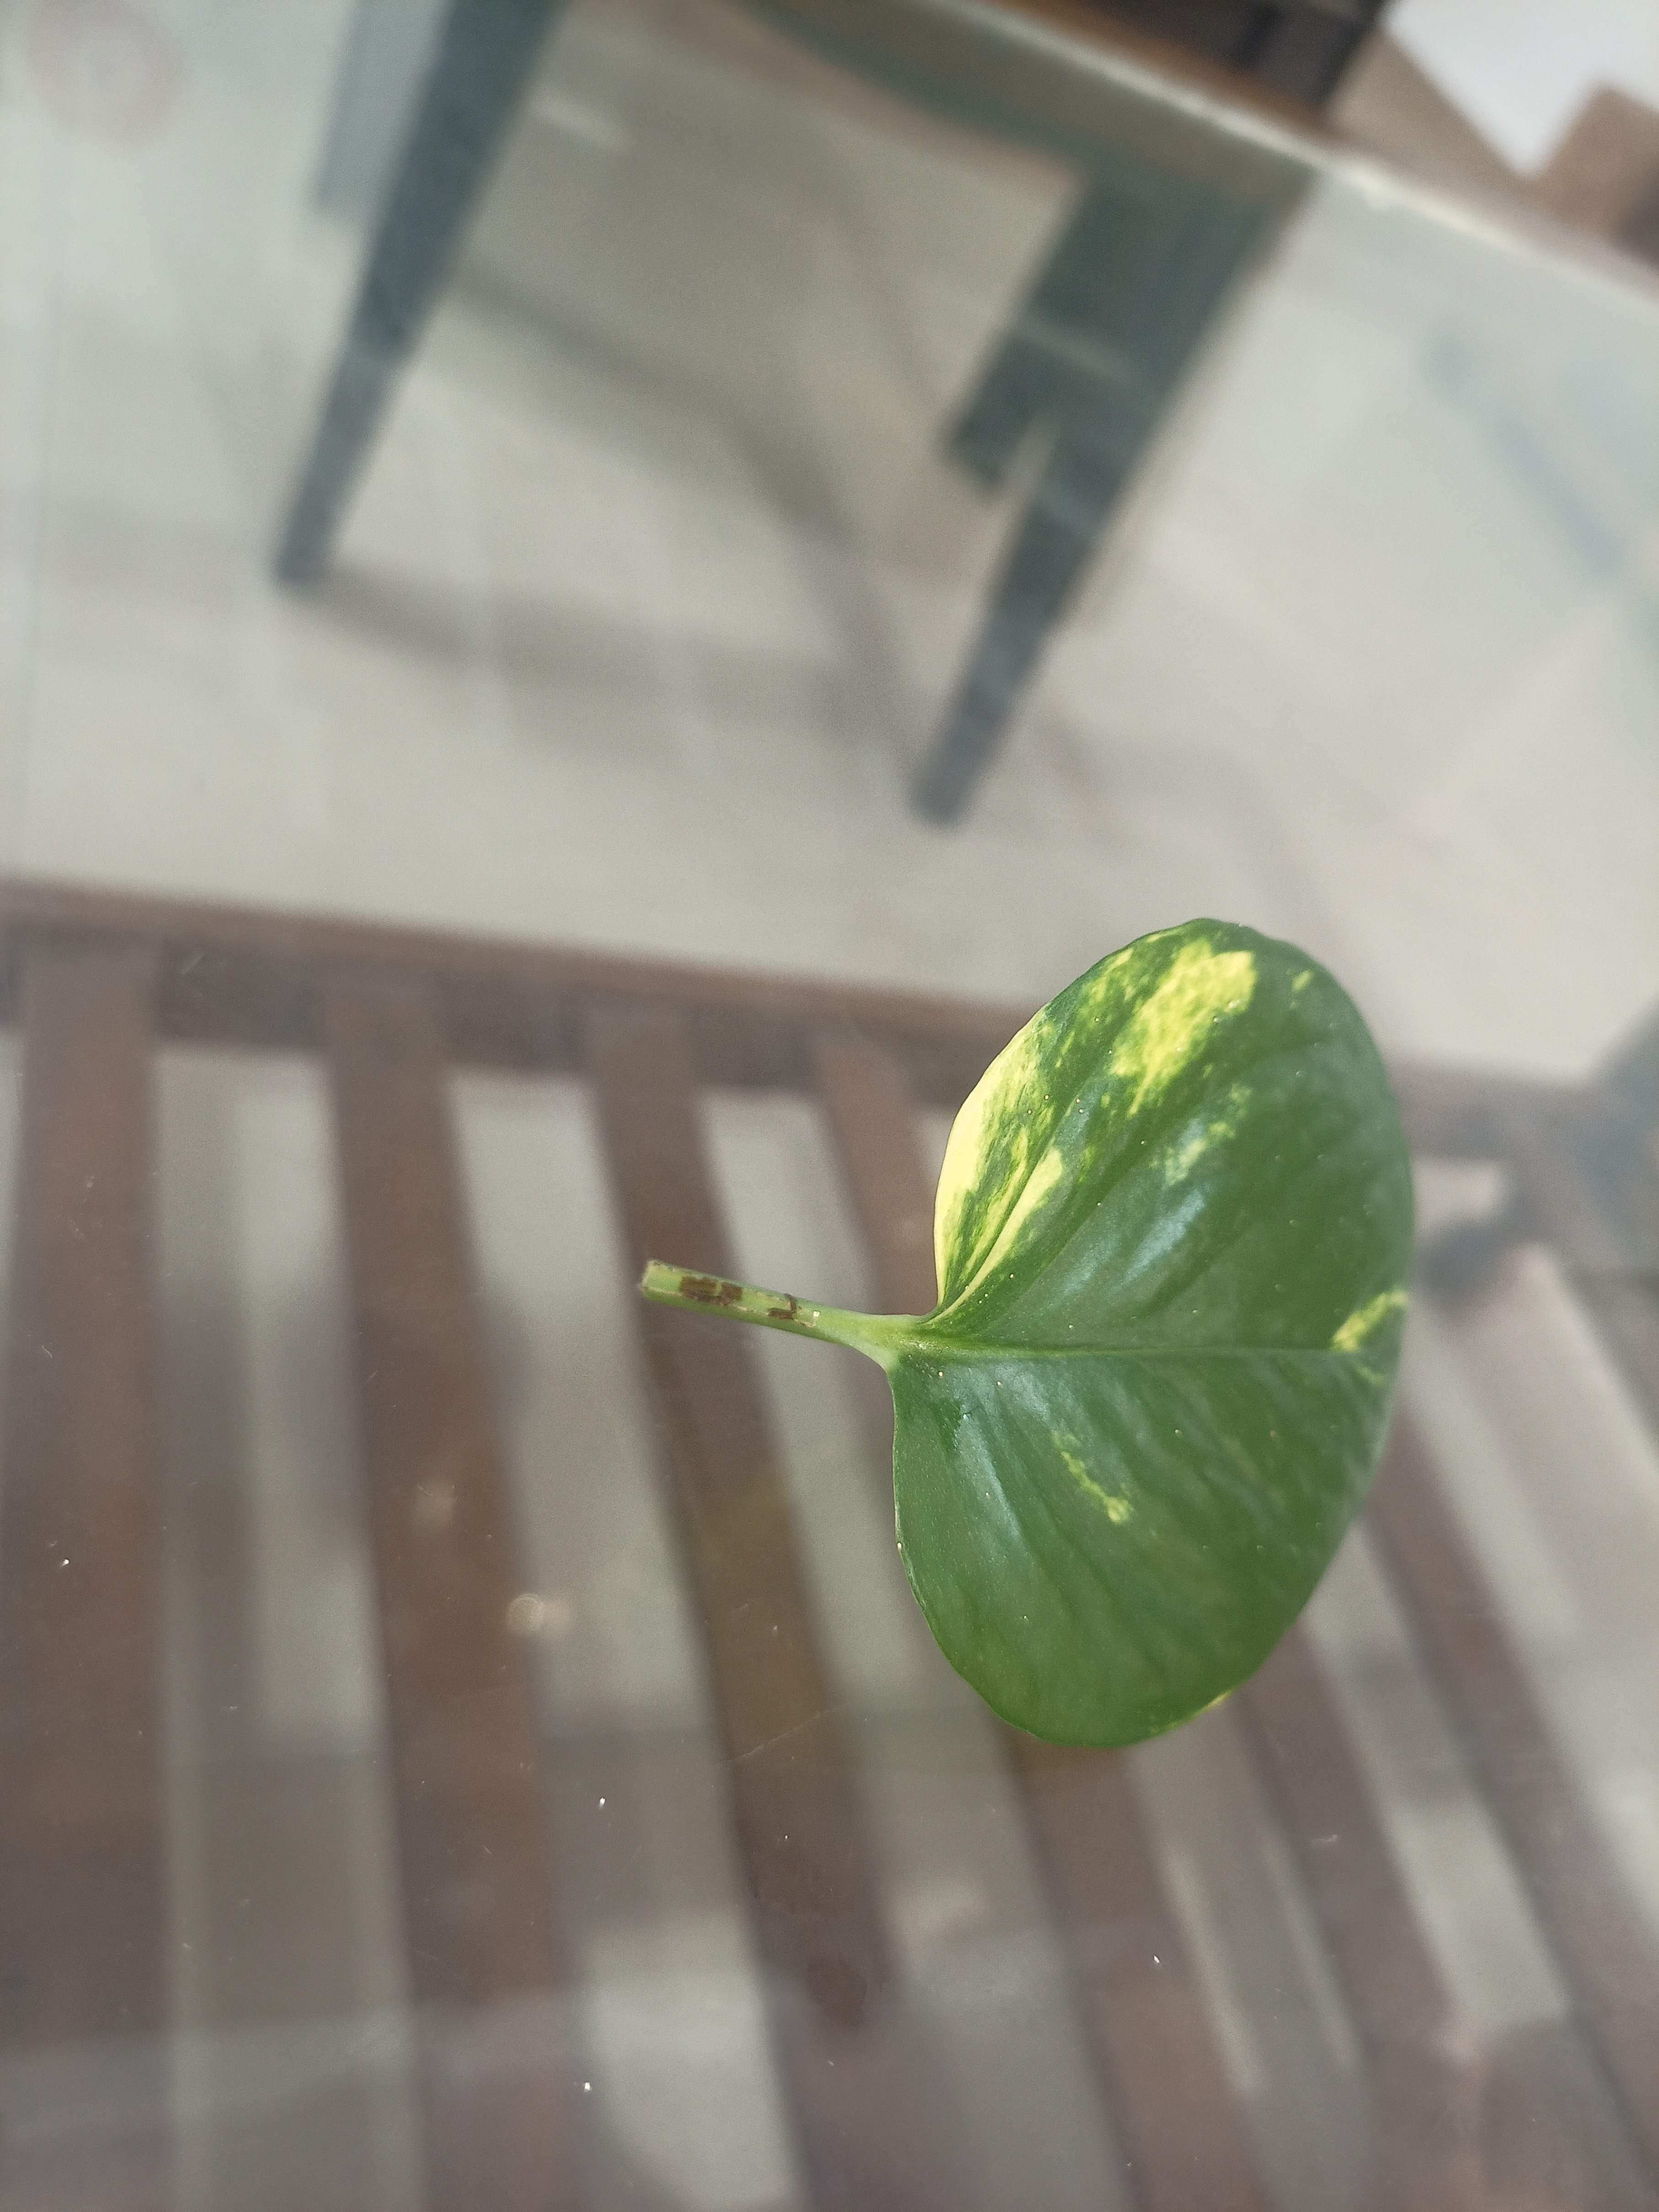
\includegraphics[width=\textwidth]{money9}
    \end{subfigure}
    \caption{Sample Money Plant leaves from the dataset}
    \label{fig:money-samples}
\end{figure}

\begin{figure}[H]
    \centering
    \begin{subfigure}[b]{0.30\columnwidth}
        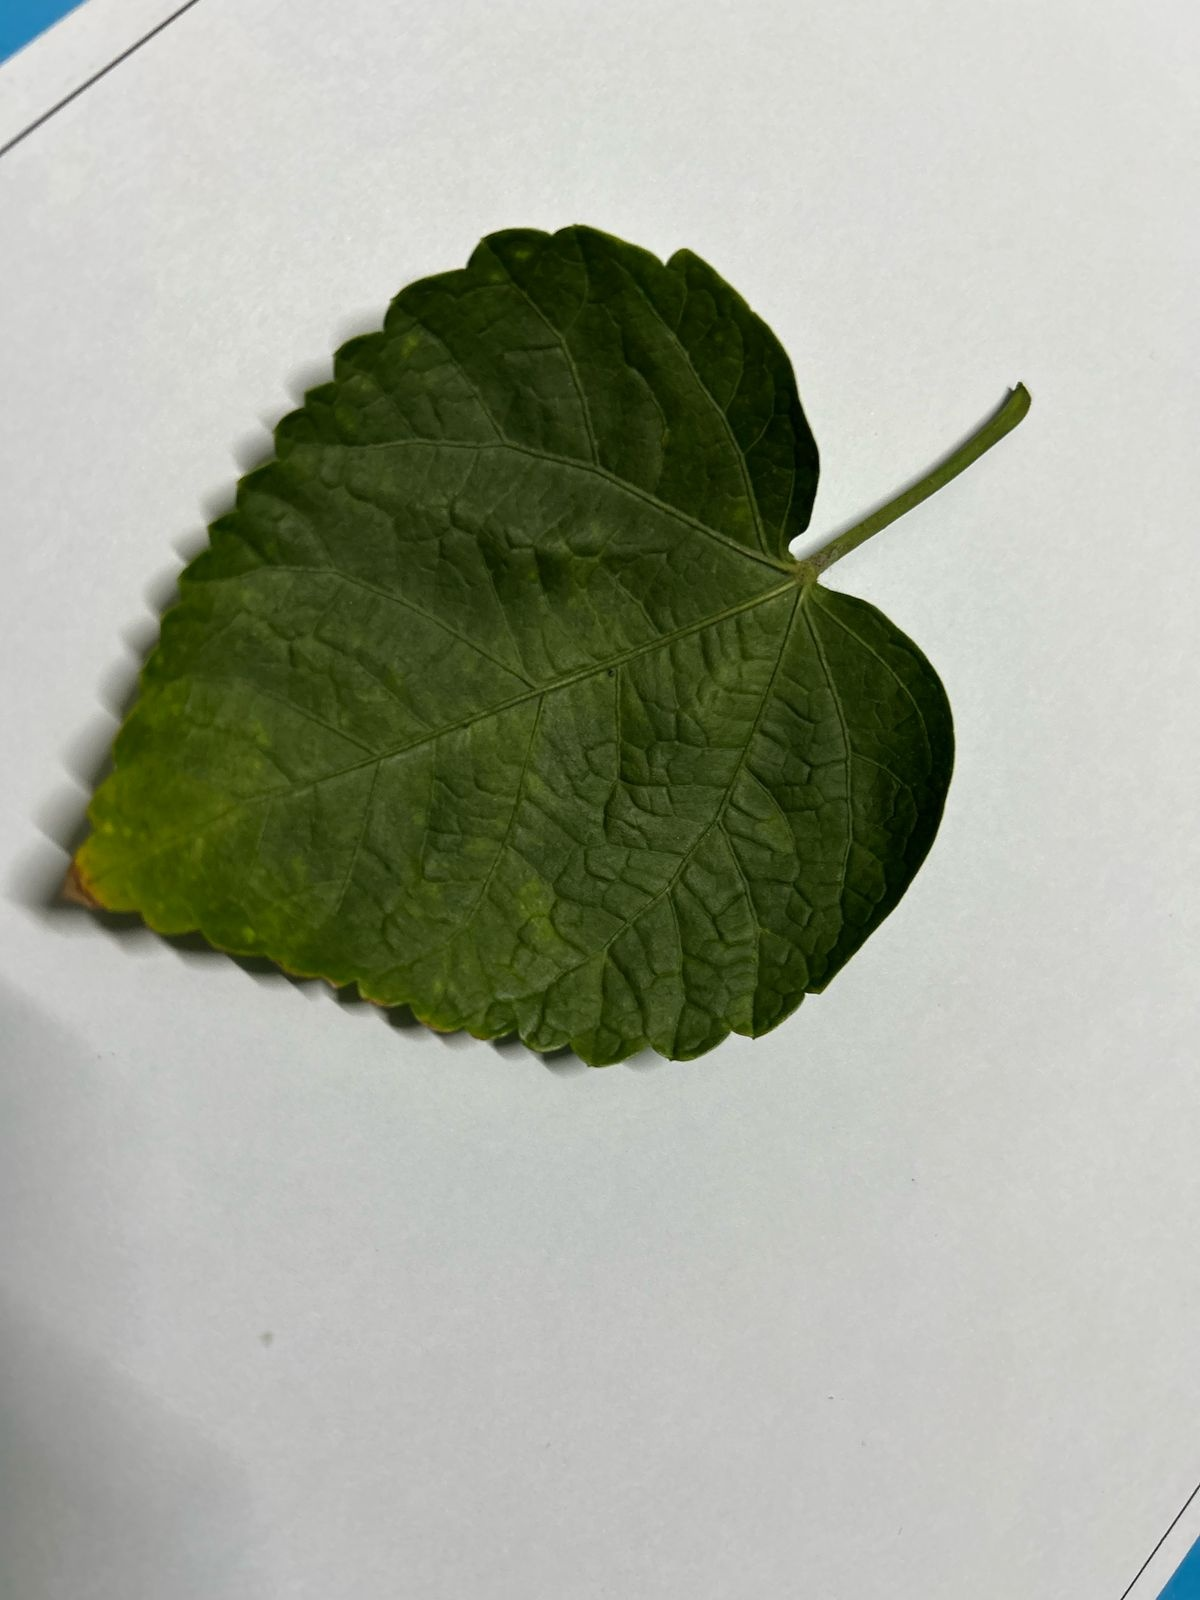
\includegraphics[width=\textwidth]{rosa1}
    \end{subfigure}
    \hfill
    \begin{subfigure}[b]{0.30\columnwidth}
        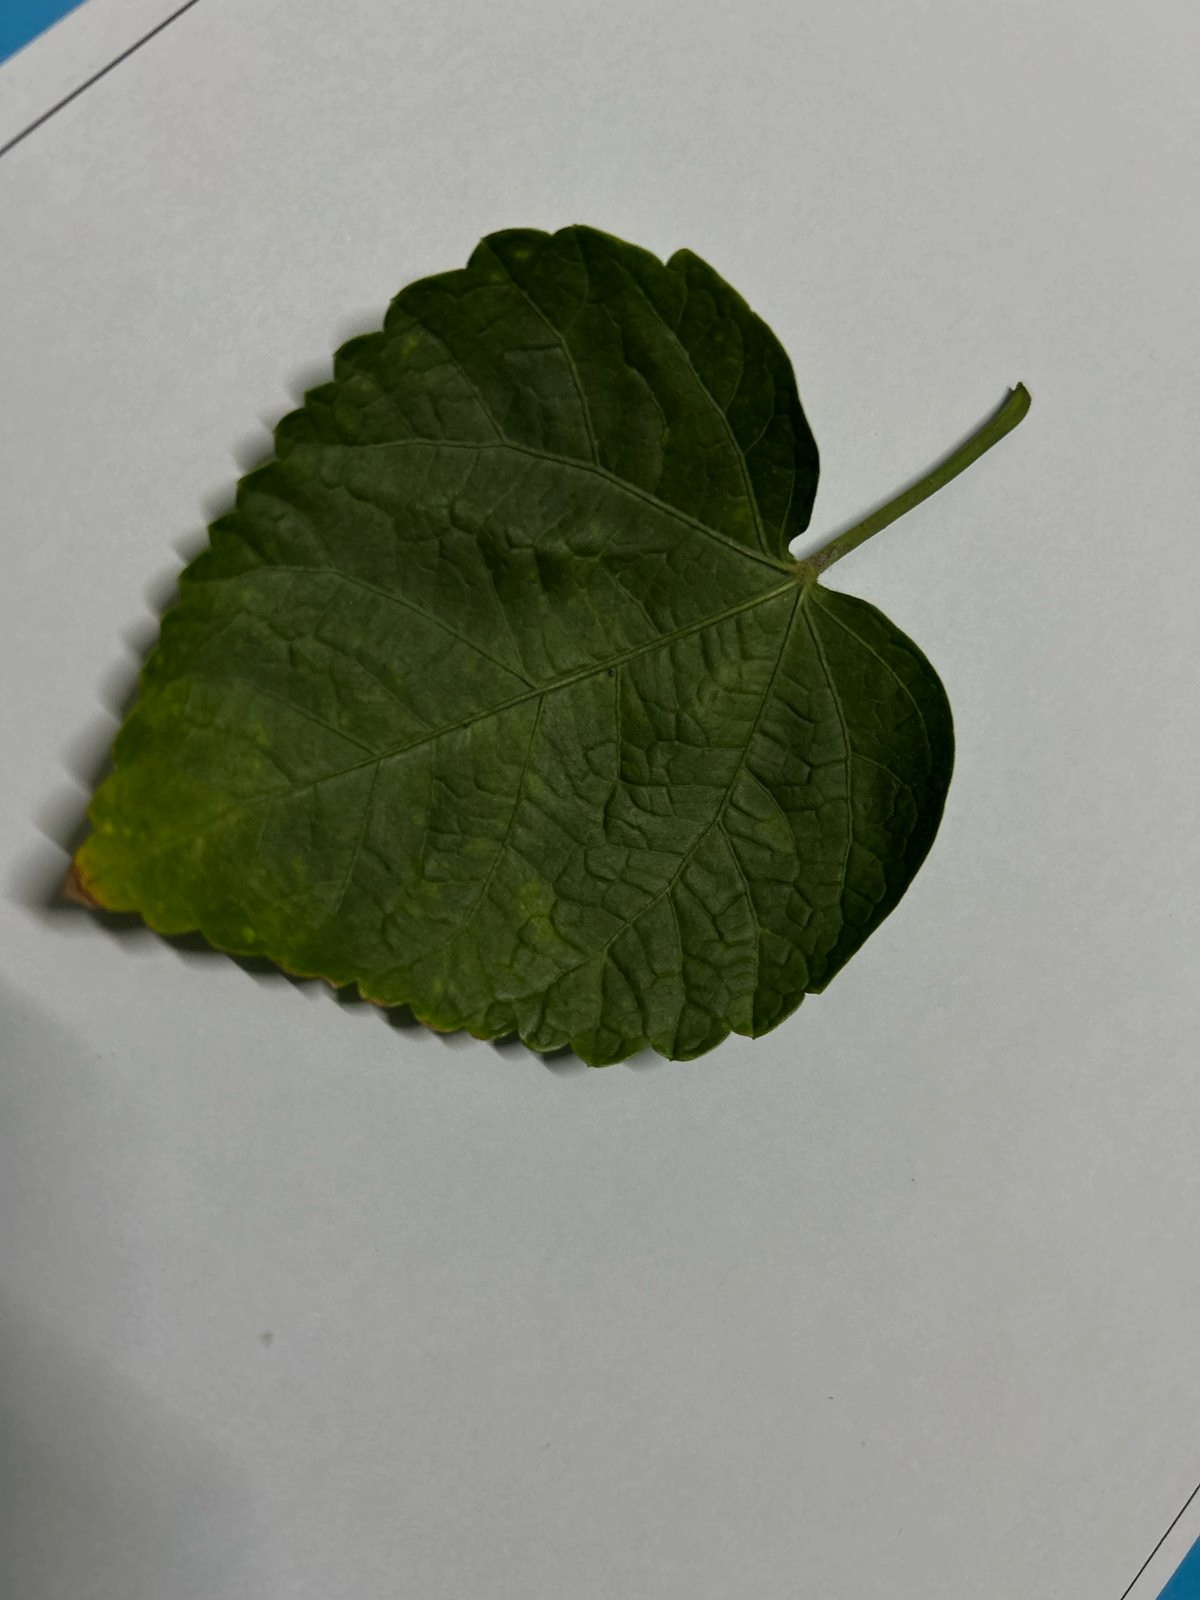
\includegraphics[width=\textwidth]{rosa2}
    \end{subfigure}
    \hfill
    \begin{subfigure}[b]{0.30\columnwidth}
        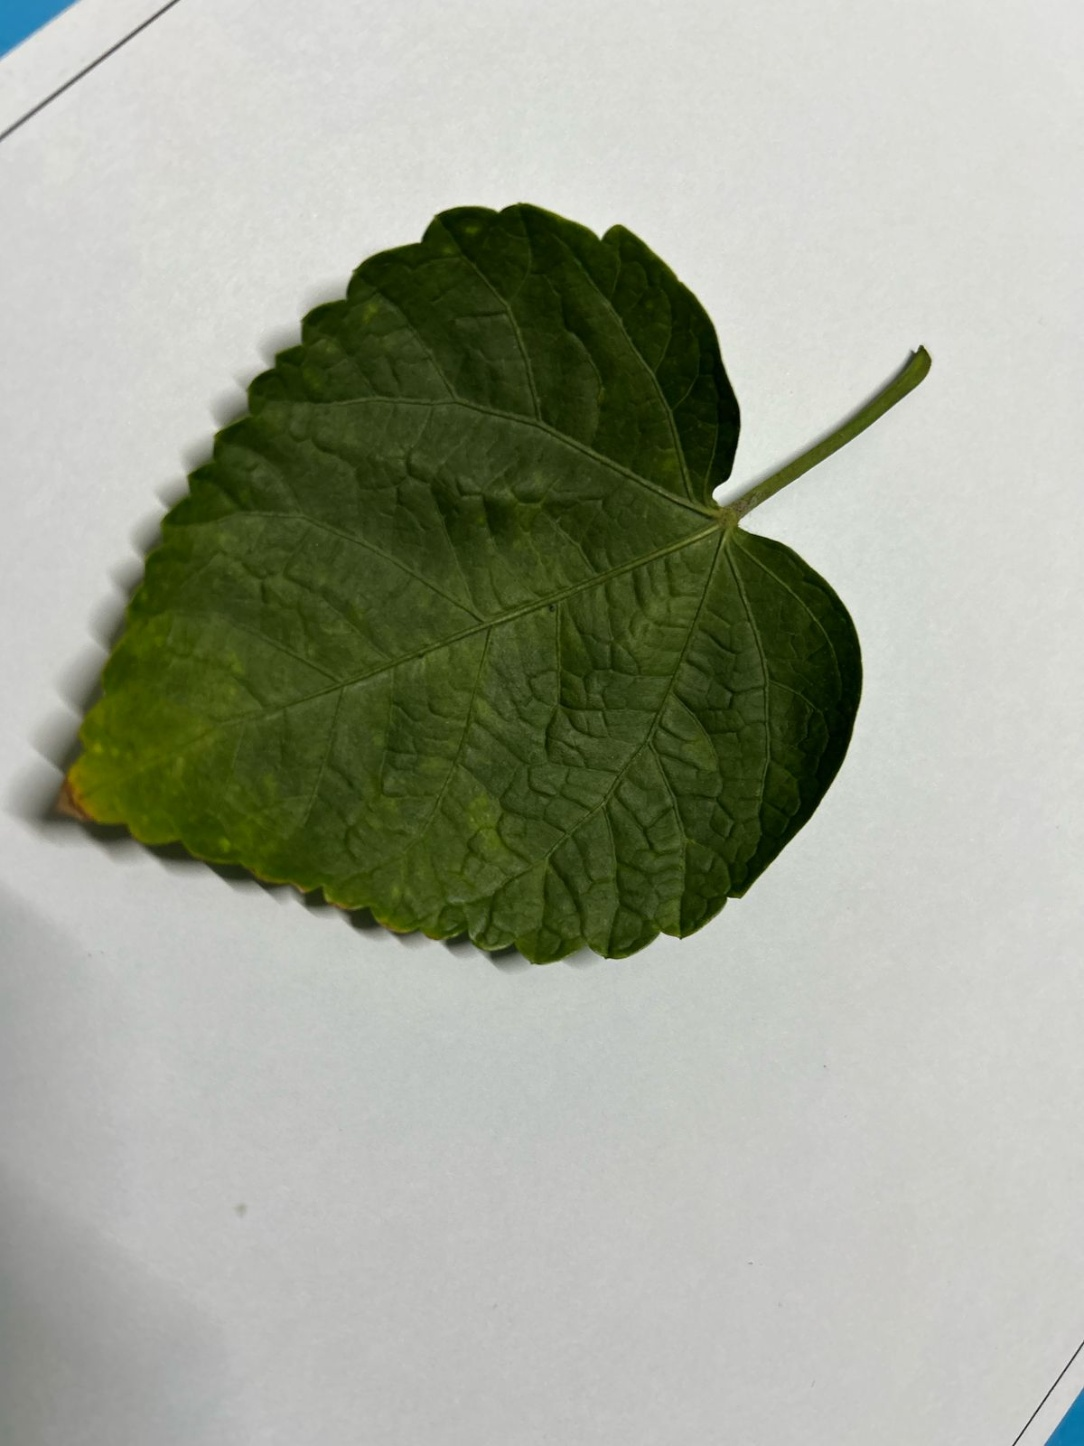
\includegraphics[width=\textwidth]{rosa3}
    \end{subfigure}
    \vspace{0.5em}
    
    \begin{subfigure}[b]{0.30\columnwidth}
        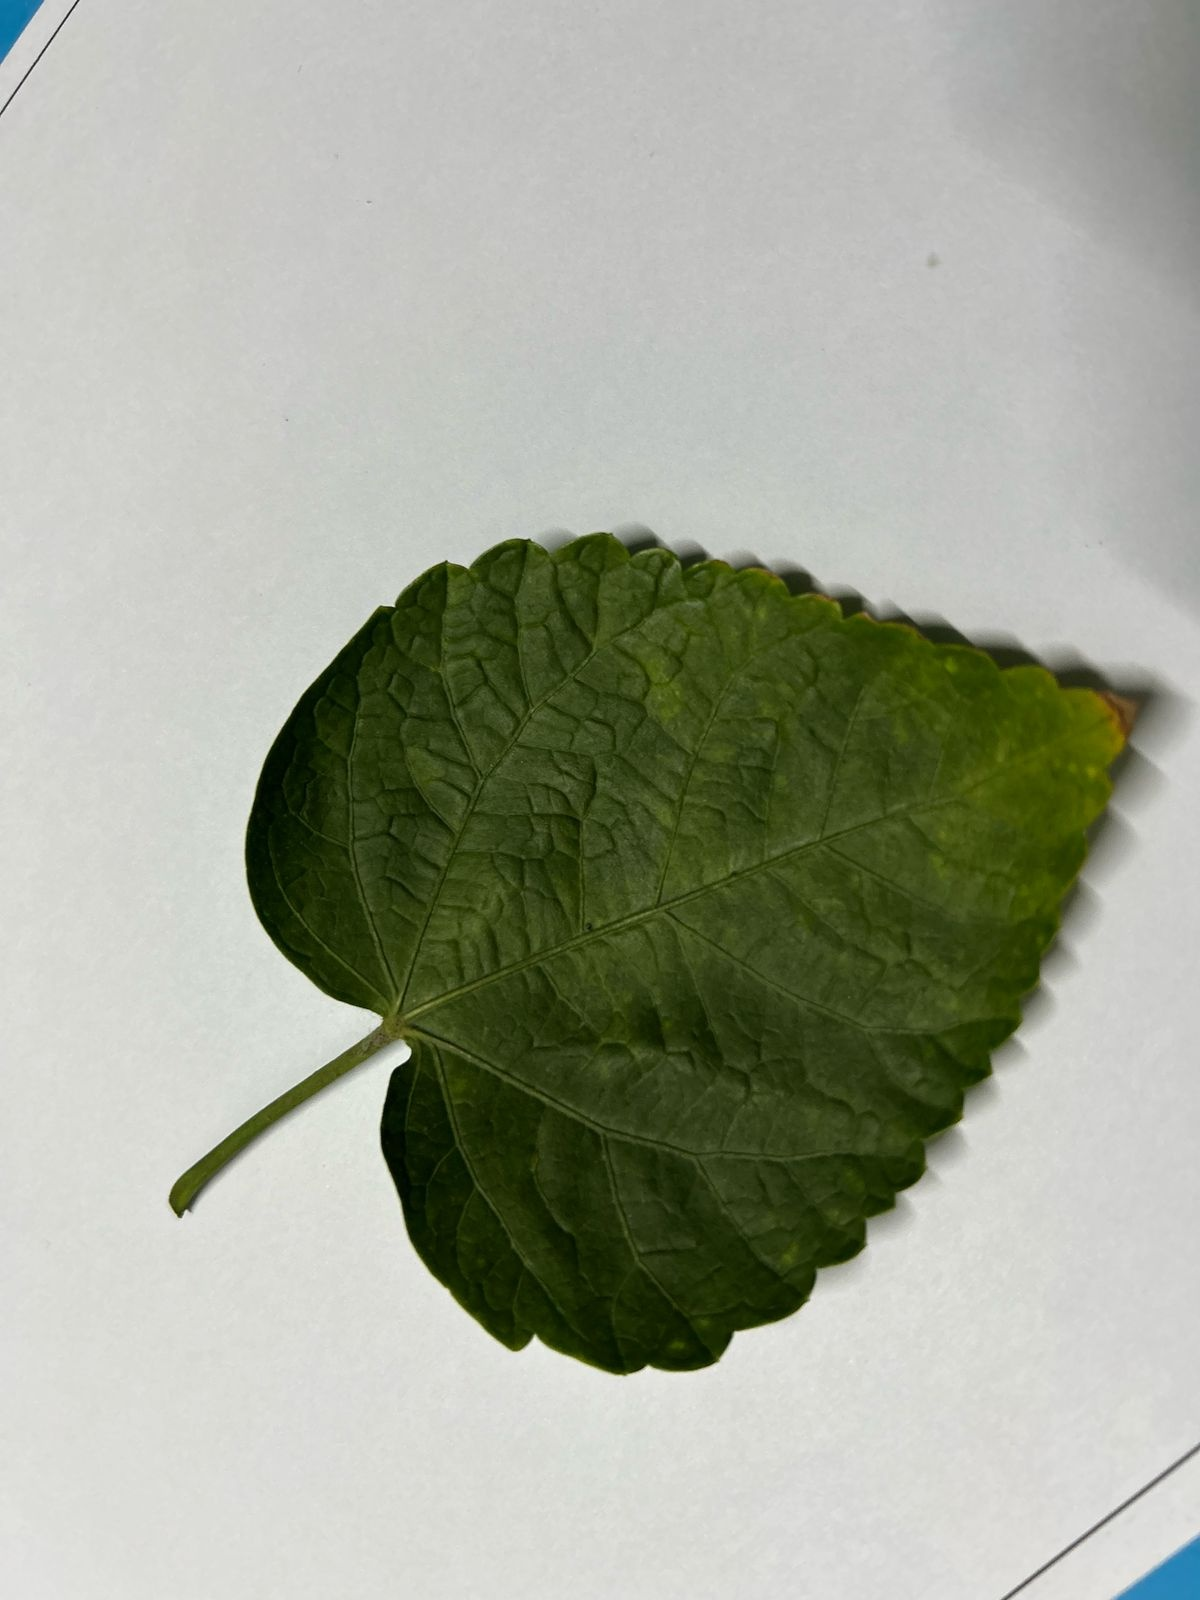
\includegraphics[width=\textwidth]{rosa4}
    \end{subfigure}
    \hfill
    \begin{subfigure}[b]{0.30\columnwidth}
        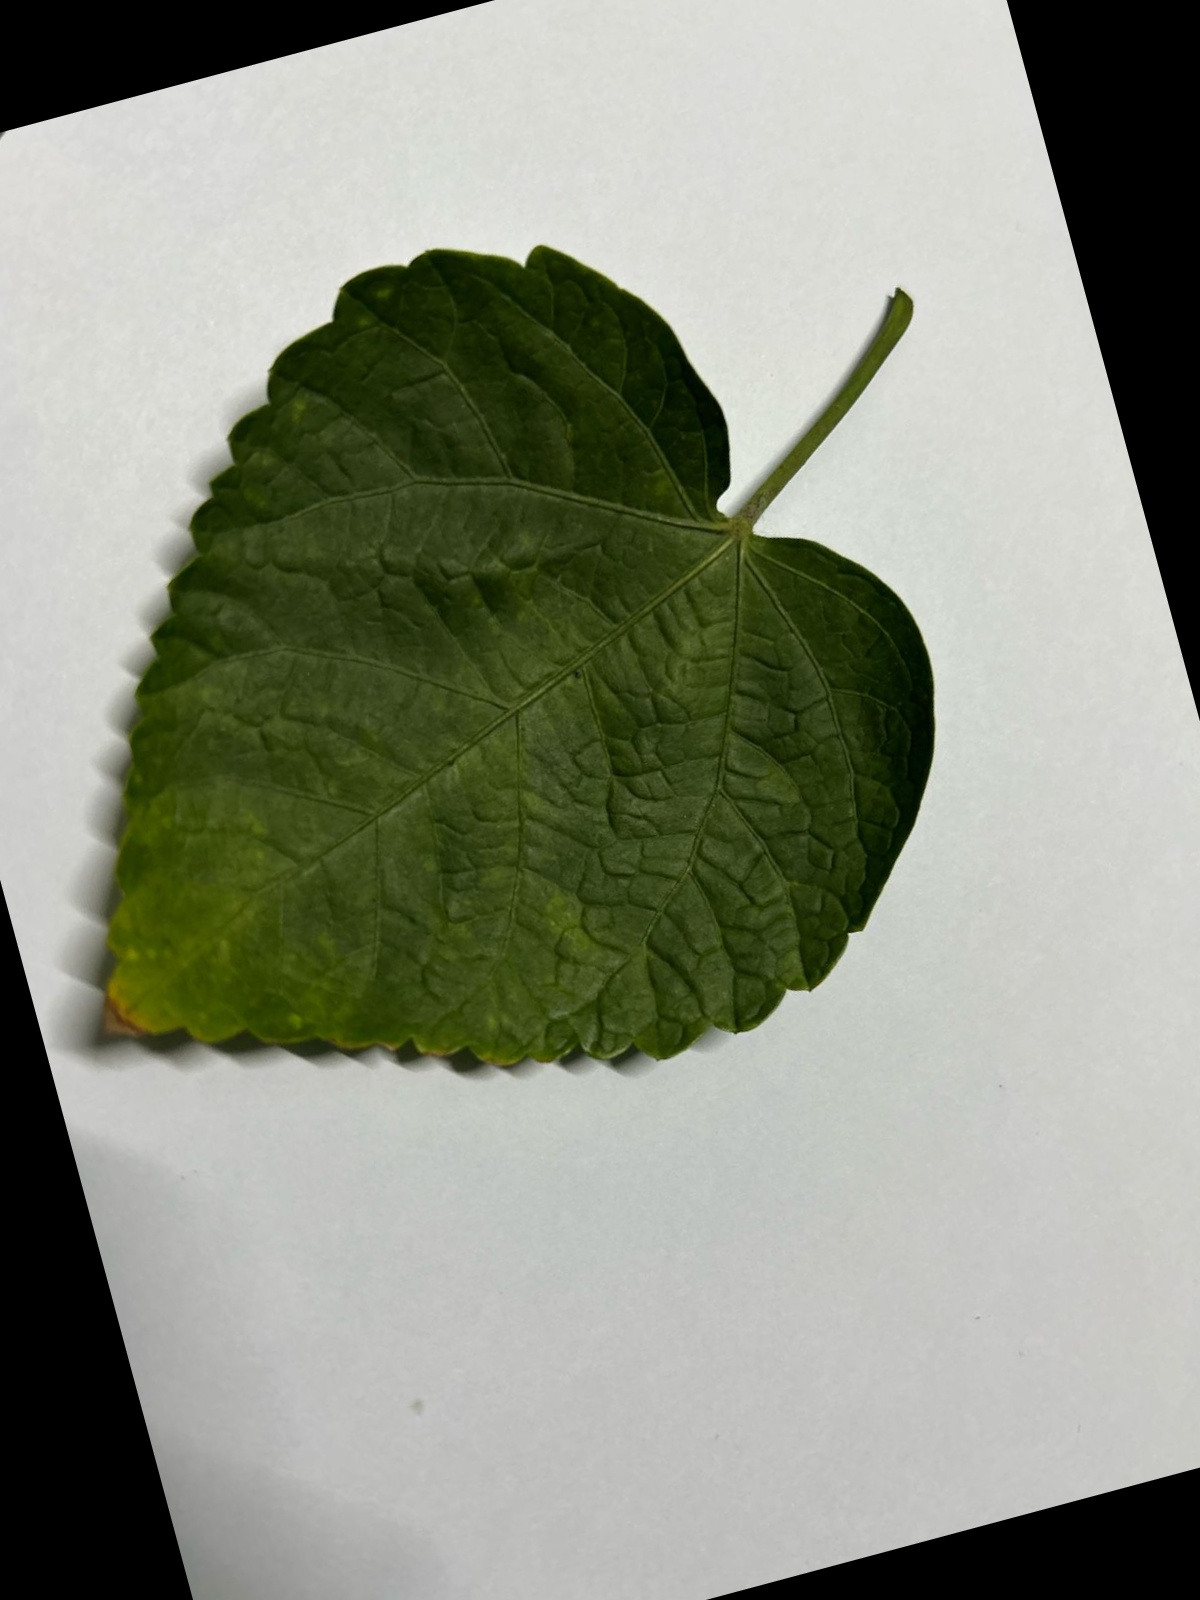
\includegraphics[width=\textwidth]{rosa5}
    \end{subfigure}
    \hfill
    \begin{subfigure}[b]{0.30\columnwidth}
        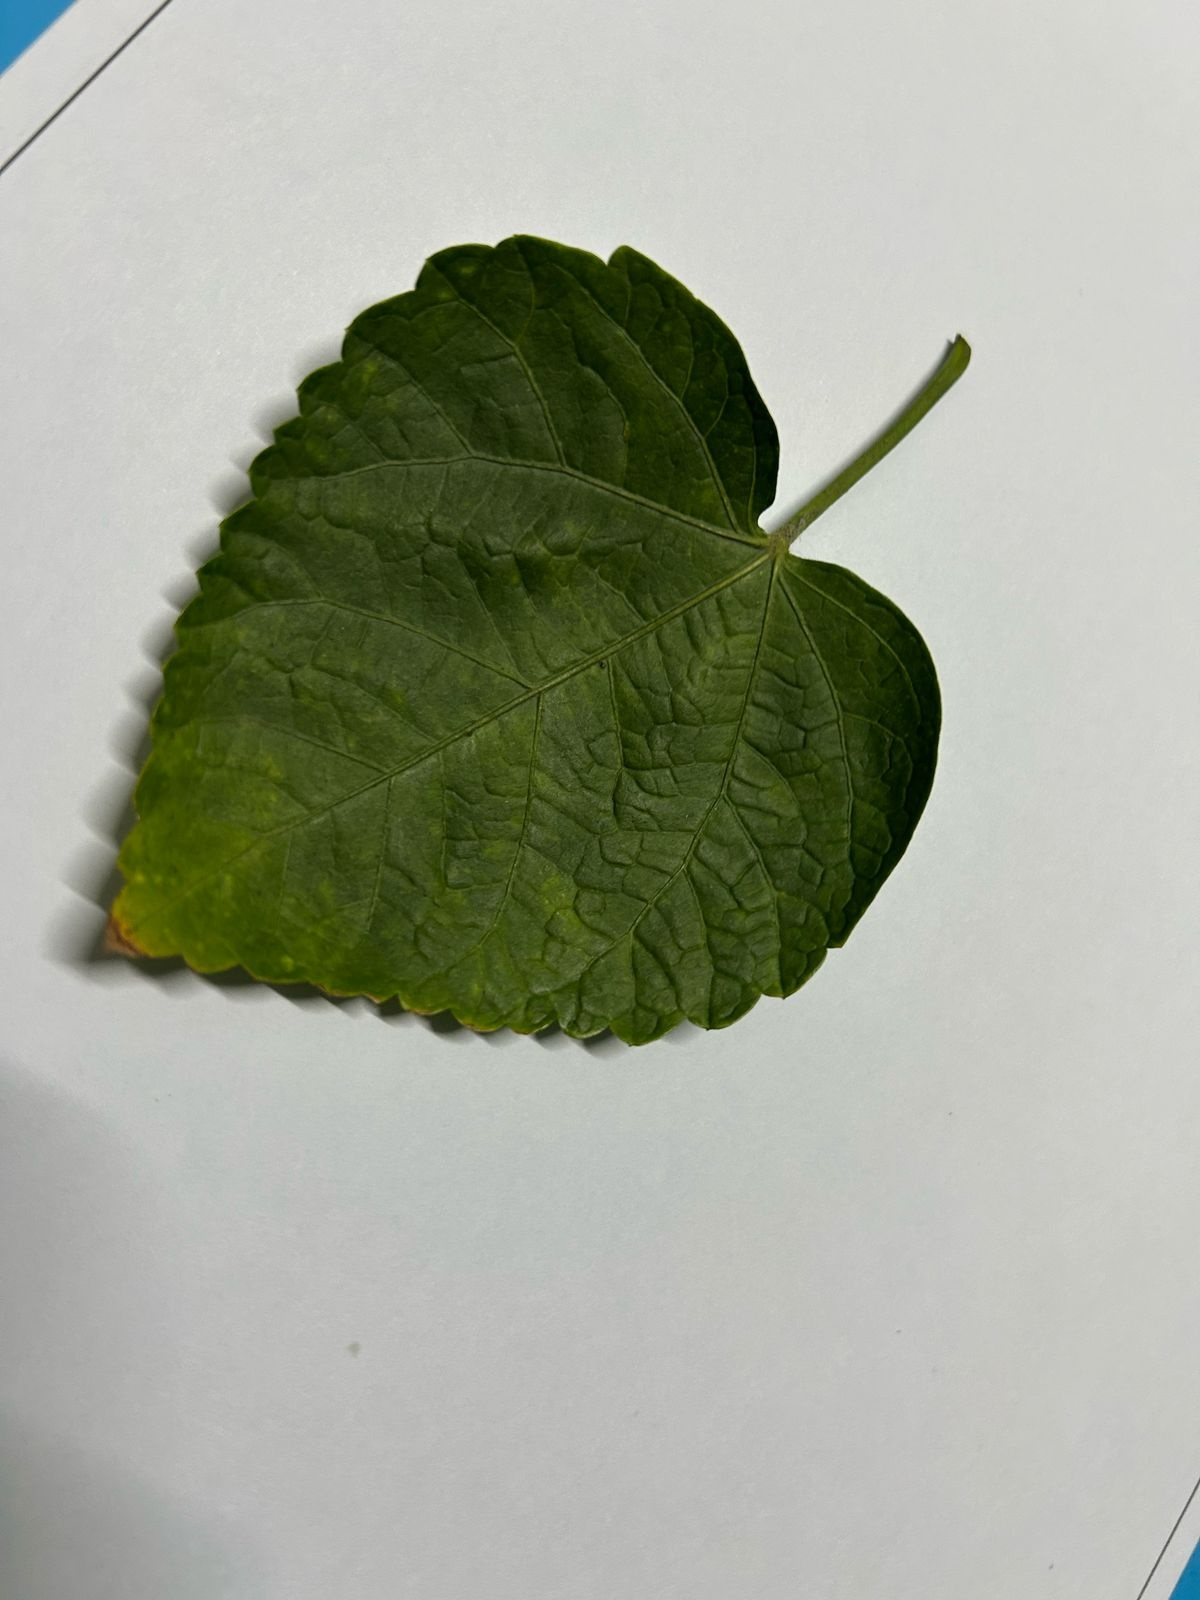
\includegraphics[width=\textwidth]{rosa6}
    \end{subfigure}
    \vspace{0.5em}
    
    \begin{subfigure}[b]{0.30\columnwidth}
        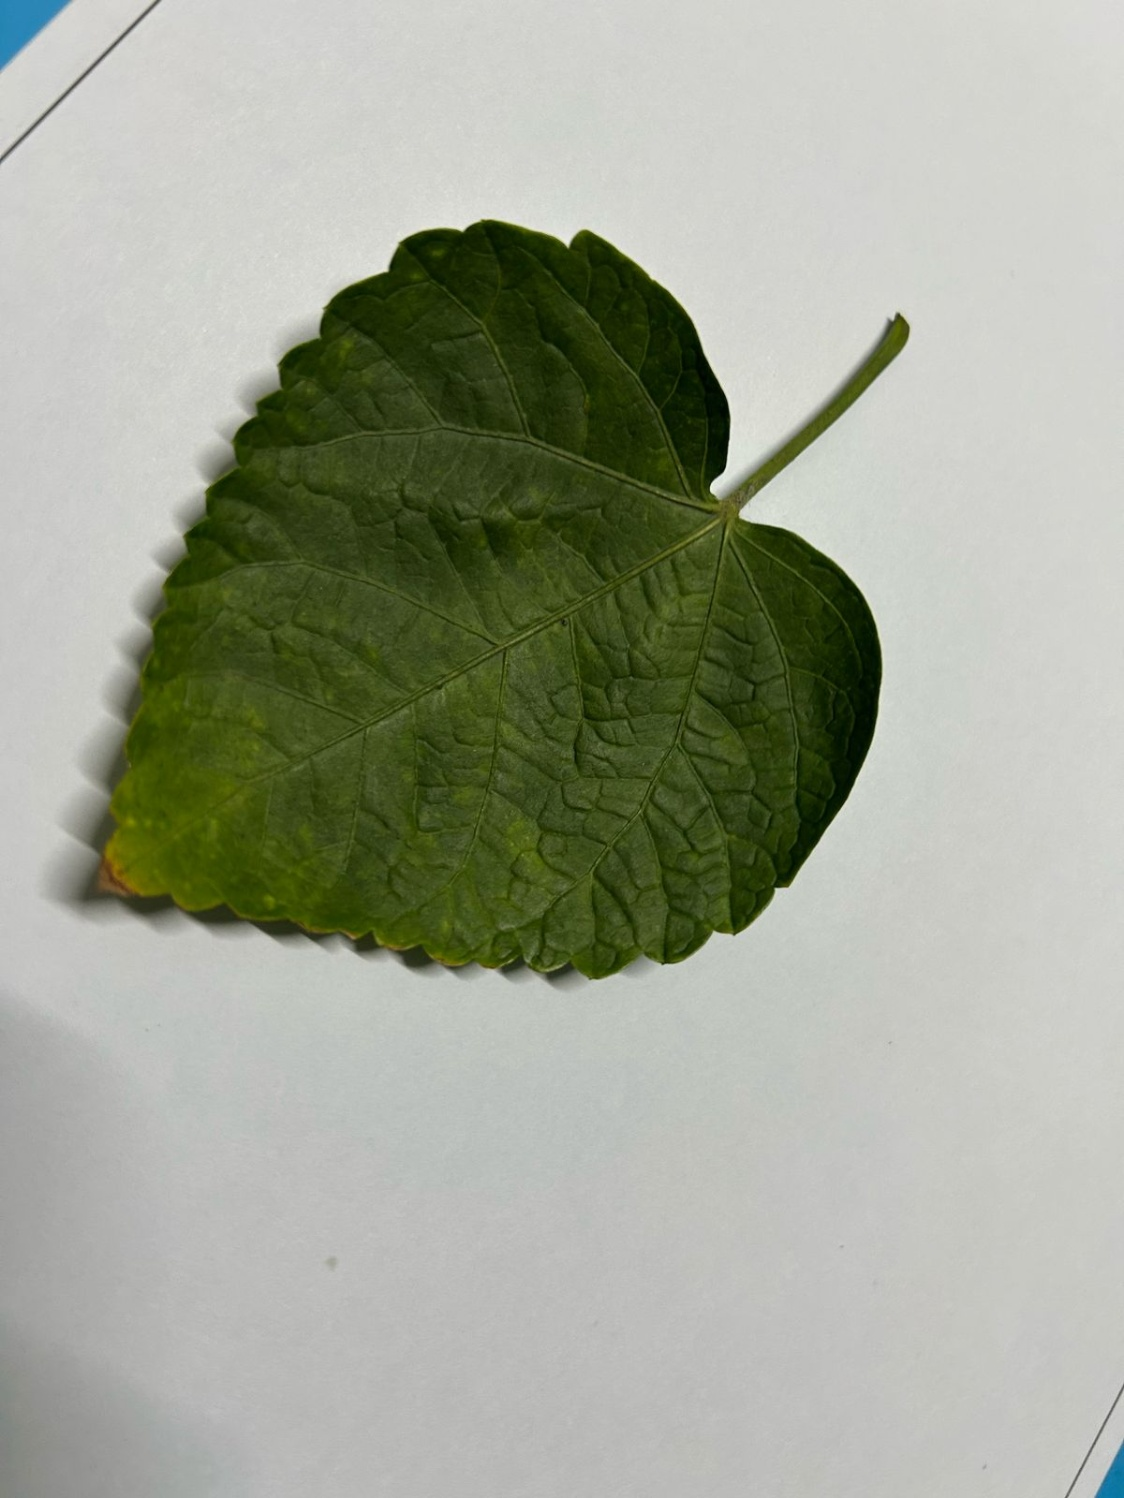
\includegraphics[width=\textwidth]{rosa7}
    \end{subfigure}
    \hfill
    \begin{subfigure}[b]{0.30\columnwidth}
        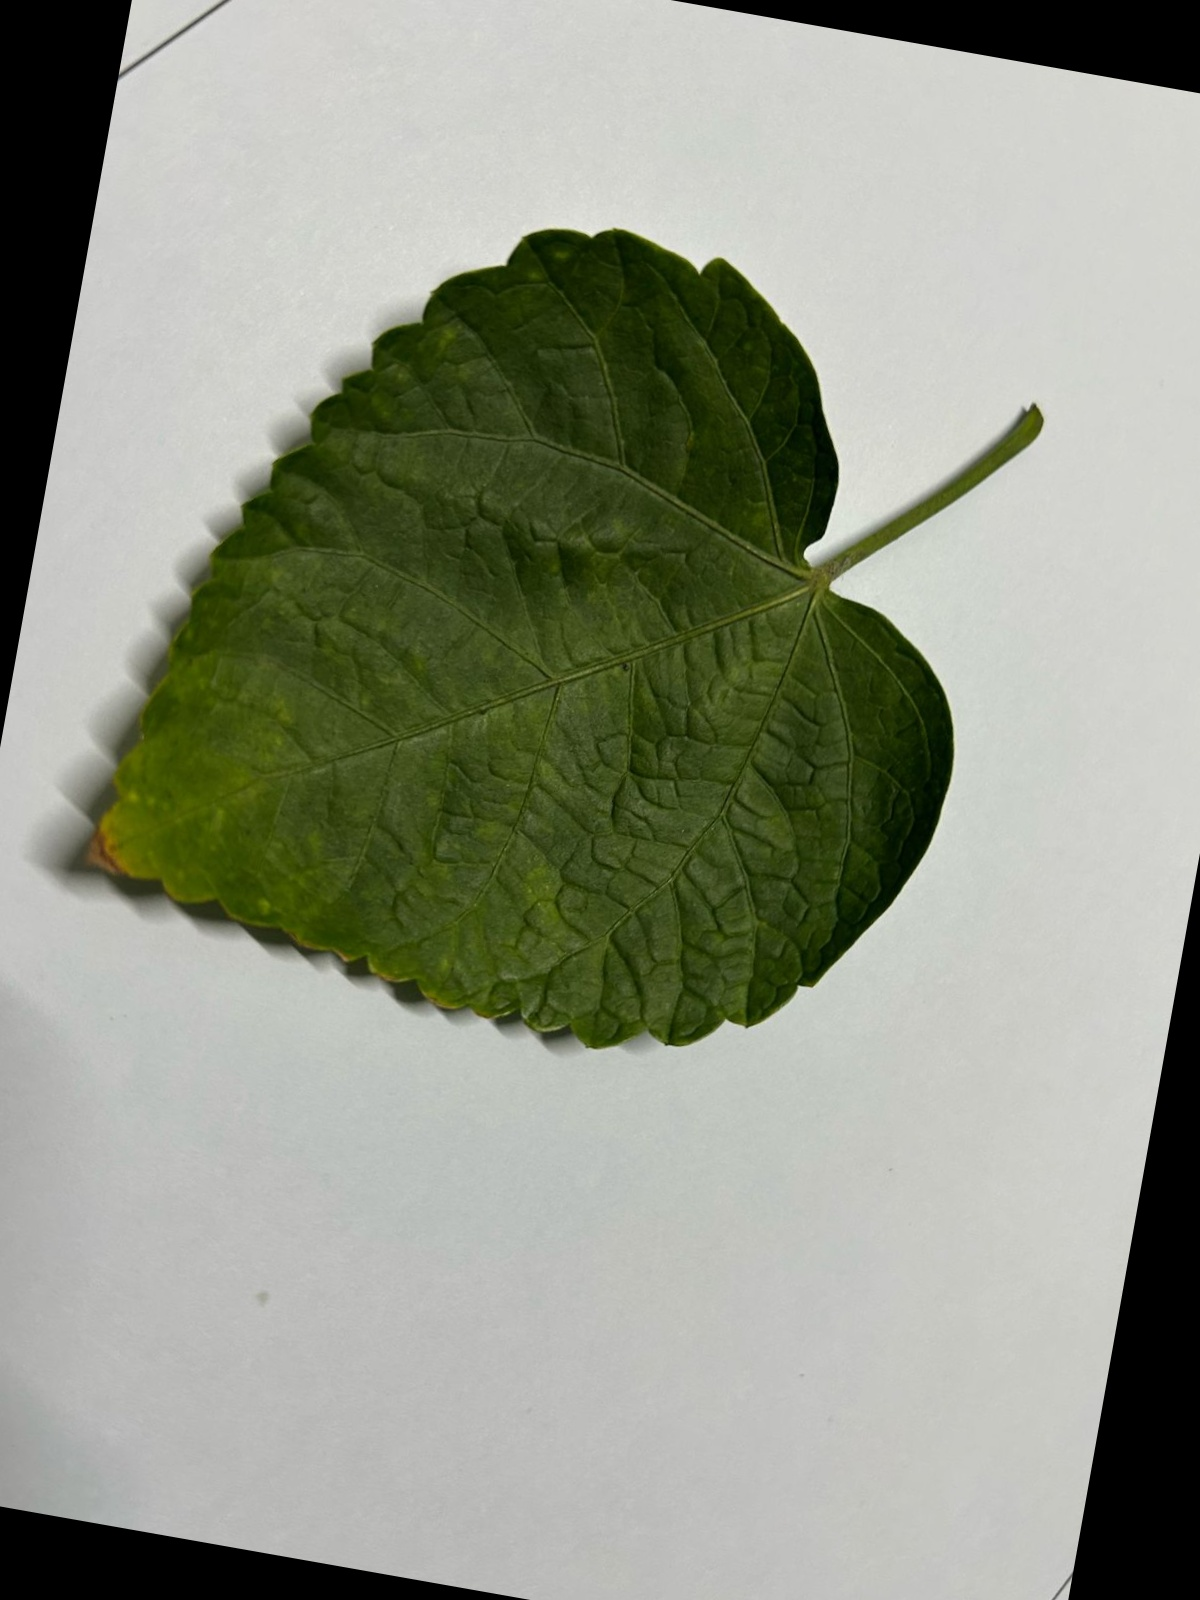
\includegraphics[width=\textwidth]{rosa8}
    \end{subfigure}
    \hfill
    \begin{subfigure}[b]{0.30\columnwidth}
        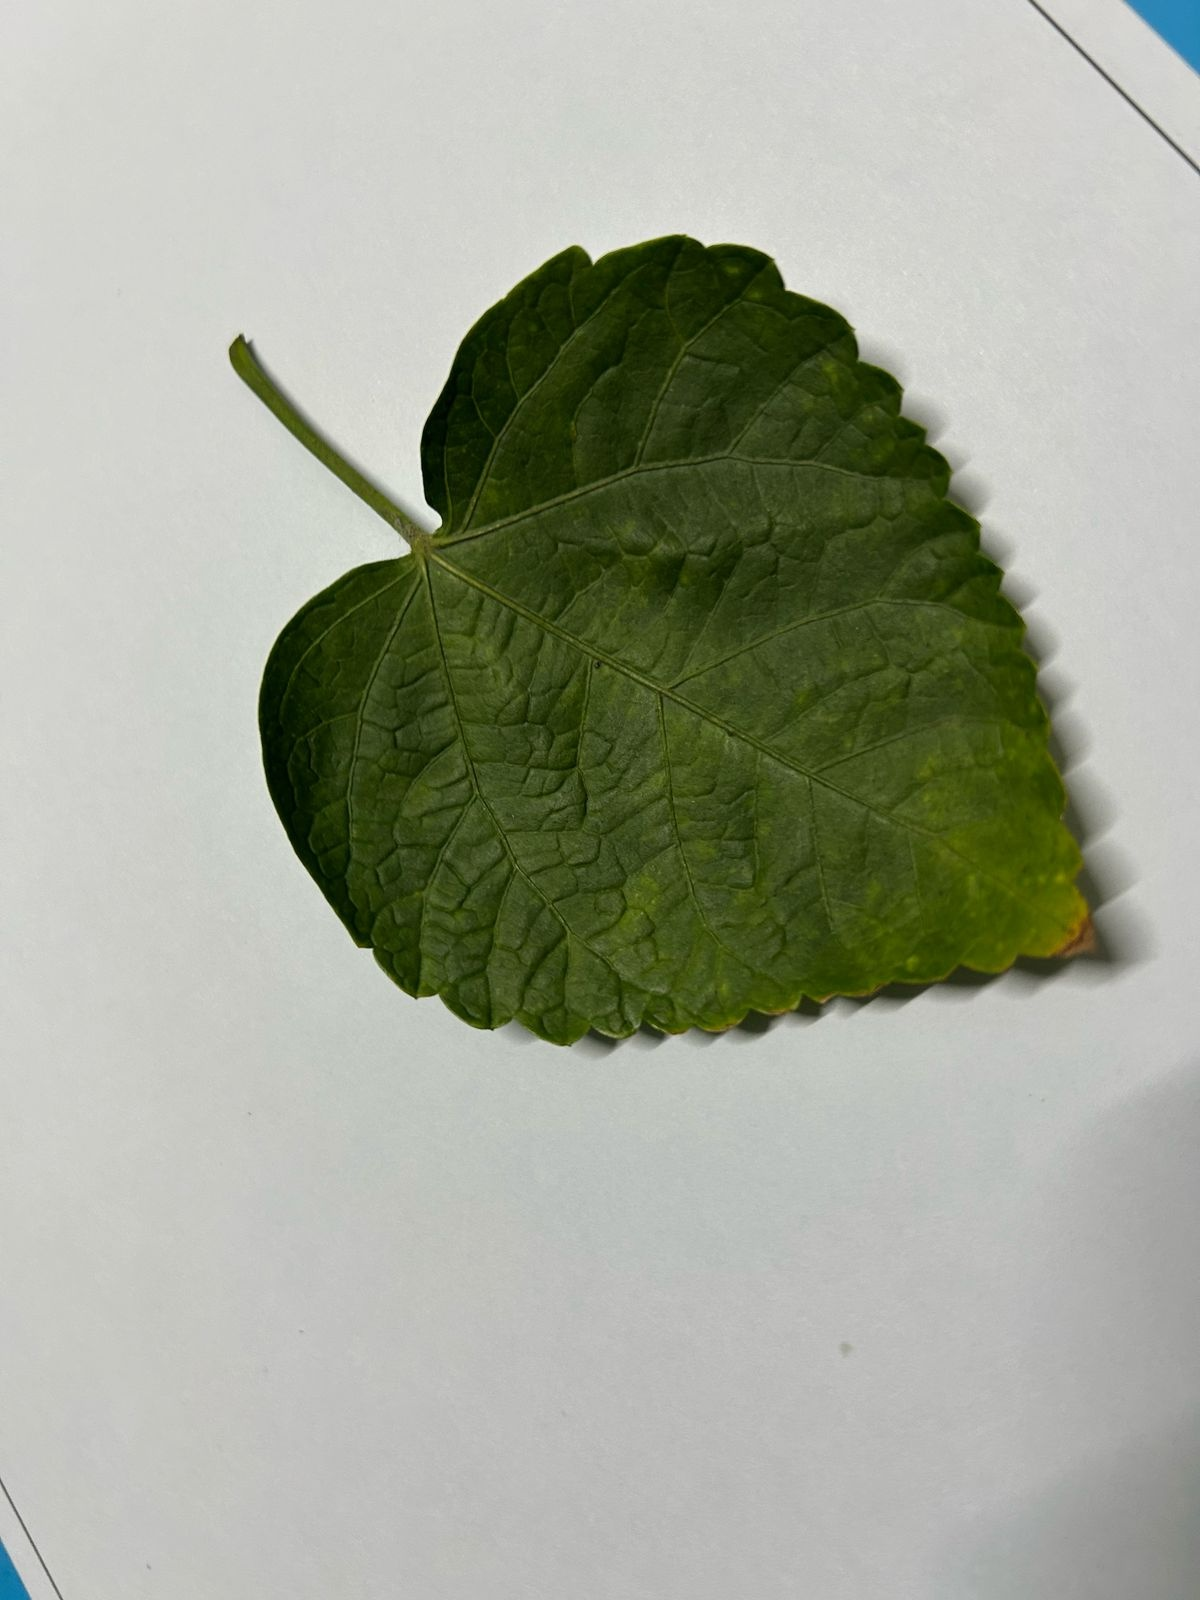
\includegraphics[width=\textwidth]{rosa9}
    \end{subfigure}
    \caption{Sample Rosa-senensis leaves from the dataset}
    \label{fig:rosa-samples}
\end{figure}

\subsection{Preprocessing}
Data preparation included:
\begin{itemize}\itemsep4pt
    \item Image Rescaling
    \item Data Augmentation:
    \begin{itemize}\itemsep2pt
        \item Rotation
        \item Flip
        \item Brightness Adjustment
    \end{itemize}
\end{itemize}

\subsection{Model Architecture}
Our custom CNN architecture consists of:
\begin{itemize}\itemsep4pt
    \item Layer 1: Conv2D (32 filters, 3×3) → ReLU → MaxPooling (2×2)
    \item Layer 2: Conv2D (64 filters, 3×3) → ReLU → MaxPooling (2×2)
    \item Layer 3: Conv2D (128 filters, 3×3) → ReLU → MaxPooling (2×2)
    \item Flatten Layer
    \item Fully Connected: Dense (256 neurons) → ReLU → Dropout (0.3)
    \item Output Layer: Dense (5 neurons) → Softmax activation
\end{itemize}

Total Parameters: 13,872,707

\section{Results}
\subsection{Model Performance}
Key metrics:
\begin{itemize}\itemsep4pt
    \item CNN Model Accuracy: 91.1\% (Test Set)
    \item Loss: 0.21 (Cross-Entropy)
    \item Training accuracy improved significantly after 10 epochs
    \item Loss decreased steadily, indicating a well-optimized model
\end{itemize}

\begin{figure}[H]
    \centering
    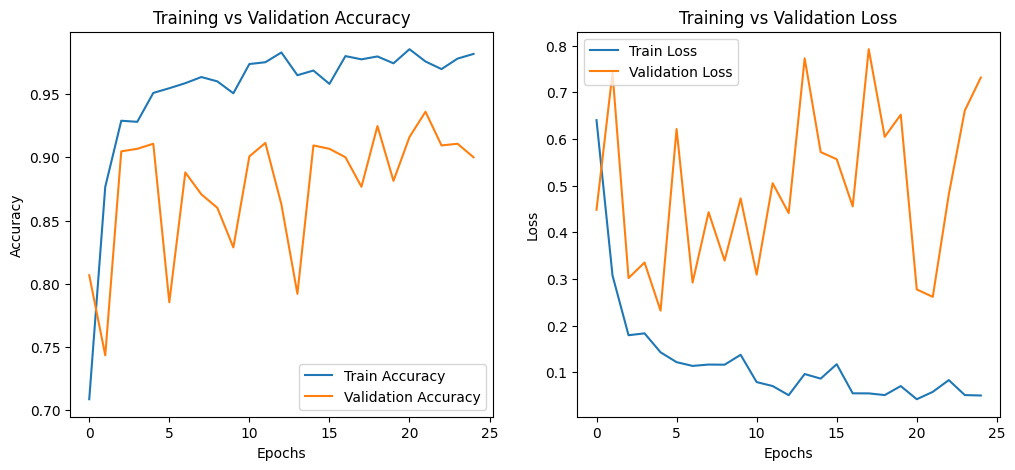
\includegraphics[width=\columnwidth]{AIML}
    \caption{Model training performance showing accuracy and loss over epochs}
    \label{fig:performance}
\end{figure}

\subsection{Analysis}
The model demonstrated strong feature extraction capabilities and effectively differentiated between species. The high accuracy achieved suggests the potential for real-world applications in botanical research and agriculture.

\section{Discussion}
The results indicate that our custom CNN model successfully classified the five species of Indian herbal plant leaves. The model's performance can be attributed to:
\begin{itemize}\itemsep4pt
    \item Effective feature extraction through multiple convolutional layers
    \item Appropriate data augmentation techniques
    \item Well-structured architecture with dropout for regularization
\end{itemize}

\section{Conclusion}
The research demonstrates the effectiveness of using custom CNNs for leaf classification. The model achieved high accuracy in classifying five species of Indian herbal plant leaves, suggesting its potential for practical applications in botanical research and agriculture.

\section*{Acknowledgments}
We would like to thank Asha M Tarsadia Institute of Computer Science and Technology for providing the necessary resources and support for this research.

\bibliographystyle{plain}
\bibliography{references}

\end{document} 